\documentclass[acmtog,review,screen,anonymous,balance=false]{acmart}
\acmSubmissionID{329}

%\usepackage{booktabs} % For formal tables

% TOG prefers author-name bib system with square brackets
\citestyle{acmauthoryear}
%\setcitestyle{nosort,square} % nosort to allow for manual chronological ordering

\usepackage[ruled]{algorithm2e} % For algorithms
\renewcommand{\algorithmcfname}{ALGORITHM}
\SetAlFnt{\small}
\SetAlCapFnt{\small}
\SetAlCapNameFnt{\small}
\SetAlCapHSkip{0pt}

% Metadata Information
\acmJournal{TOG}
%\acmVolume{38}
%\acmNumber{4}
%\acmArticle{39}
%\acmYear{2019}
%\acmMonth{7}

% Copyright
%\setcopyright{acmcopyright}
%\setcopyright{acmlicensed}
%\setcopyright{rightsretained}
%\setcopyright{usgov}
%\setcopyright{usgovmixed}
%\setcopyright{cagov}
%\setcopyright{cagovmixed}

% DOI
%\acmDOI{0000001.0000001_2}

\settopmatter{printacmref=false} % Removes citation information below abstract
\renewcommand\footnotetextcopyrightpermission[1]{} % Removes footnote with conference information in first column

\usepackage{ifthen}
\usepackage{mathtools}
% \usepackage[usenames,dvipsnames]{xcolor}
% \usepackage{multirow,pbox}
\usepackage{multirow}
\usepackage{nicefrac}
\usepackage[many]{tcolorbox}
\usepackage{comment,xspace}
\usepackage{accents}
\usepackage{enumitem}
\usepackage{overpic}
\setlist[itemize]{parsep=0pt,partopsep=0pt,leftmargin=*,itemsep=5pt}
\setlist[enumerate]{parsep=0pt,partopsep=0pt,leftmargin=*,itemsep=5pt}

\newlength{\resLen}
\newlength{\resLenTwo}
\newlength{\raiseLen}

%%%%%%%%%%%%%%%%%%%%
% Marcos for other symbols
%%%%%%%%%%%%%%%%%%%%

\renewcommand{\to}{\shortrightarrow}

\newcommand{\defeq}{\vcentcolon=}
\newcommand{\eqdef}{=\vcentcolon}
%
% \stackMath
% \newcommand\reallywidehat[1]{%
% \savestack{\tmpbox}{\stretchto{%
%   \scaleto{%
%     \scalerel*[\widthof{\ensuremath{#1}}]{\kern-.6pt\bigwedge\kern-.6pt}%
%     {\rule[-\textheight/2]{1ex}{\textheight}}%WIDTH-LIMITED BIG WEDGE
%   }{\textheight}% 
% }{0.5ex}}%
% \stackon[1pt]{#1}{\tmpbox}%
% }
\makeatletter
\newcommand{\dotr}[1]{%
	\mathpalette\@dotr{#1}%
}
\newcommand*{\@dotr}[2]{%
	% #1: math style (\displaystyle, ..., \scriptscriptstyle)
	% #2: argument of \dotr
	\sbox0{$\m@th#1#2$}%
	\usebox{0}%
	% simulating a superscript
	\raisebox{\dimexpr\ht0-\height}{$\m@th#1\@smallbullet#1\bullet$}%
	\kern\scriptspace
}
\newcommand*{\@smallbullet}[2]{%
	\scalebox{.4}{$\m@th#1#2$}%
}
\makeatother

\newcommand{\bd}{\boldsymbol{d}}
\newcommand{\bu}{\boldsymbol{u}}
\newcommand{\bx}{\boldsymbol{x}}
\newcommand{\by}{\boldsymbol{y}}
\newcommand{\bz}{\boldsymbol{z}}
\newcommand{\bn}{\boldsymbol{n}}
\newcommand{\bp}{\boldsymbol{p}}
\newcommand{\bq}{\boldsymbol{q}}
\newcommand{\be}{\boldsymbol{e}}
\newcommand{\bv}{\boldsymbol{v}}
\newcommand{\bI}{\boldsymbol{I}}
\newcommand{\bom}{\boldsymbol{\omega}}

\newcommand{\Real}{\mathbb{R}}
\newcommand{\bbS}{\mathbb{S}}
\newcommand{\Sph}{\bbS^2}
\newcommand{\vis}{\mathbb{V}}
\newcommand{\bbP}{\mathbb{P}}

\newcommand{\Le}[1][]{L_{\ifthenelse{\equal{#1}{}}{\mathrm{e}}{\mathrm{e},#1}}}
\newcommand{\Li}{L_\mathrm{i}}
\newcommand{\Lr}{L_\mathrm{r}}
\newcommand{\We}{W_\mathrm{e}}
\newcommand{\bWe}{\boldsymbol{W}_\mathrm{e}}
\newcommand{\Ae}{A_\mathrm{e}}
\newcommand{\bAe}{\boldsymbol{A}_\mathrm{e}}

\newcommand{\bomi}{\bom_\mathrm{i}}
\newcommand{\bomo}{\bom_\mathrm{o}}
\newcommand{\bxo}{\bx_\mathrm{o}}
\newcommand{\bsdf}{f_\mathrm{s}}

\newcommand{\sigS}{\sigma_\mathrm{s}}
\newcommand{\sigA}{\sigma_\mathrm{a}}
\newcommand{\sigT}{\sigma_\mathrm{t}}
\newcommand{\phase}{f_\mathrm{p}}
\newcommand{\cS}{C_\mathrm{s}}
\newcommand{\cA}{C_\mathrm{a}}
\newcommand{\cT}{C_\mathrm{t}}

\newcommand{\dtheta}{\dir{\boldsymbol\theta}}
\newcommand{\dphi}{\dir{\boldsymbol\dphi}}

\newcommand{\newdef}[2]{%
    \hypertarget{label:def:#1}{\textbf{#2}}%
}

\newcommand{\refdef}[2]{%
    %\hyperlink{label:def:#1}{\textcolor{ACMPurple}{#2}}%
    \hyperlink{label:def:#1}{\textcolor{gray}{#2}}%
}

\newcommand{\gy}[1]{\textcolor{red}{[\textbf{Yu:} {\em #1}]}}
\newcommand{\sz}[1]{\textcolor{blue}{[\textbf{SZ:} {\em #1}]}}

\newcommand{\AJ}[1]{\textcolor{green}{[\textbf{AJ:} {\em #1}]}}

%%%%%%%%%%%%%%%%%%%%%%%%%%%%%%%%%%%%%%%%%%%%%%%%%%%%%%%%%%%%%%%%%%%%%
% EM-Based scattering macros (symbols now follow [Mischenko 2002], can
% be changed to something more common in graphics
%%%%%%%%%%%%%%%%%%%%%%%%%%%%%%%%%%%%%%%%%%%%%%%%%%%%%%%%%%%%%%%%%%%%%
\newcommand{\dir}[1]{\mathbf{\hat{#1}}}

\newcommand{\px}{\mathbf{r}}
\newcommand{\dpx}{\dir{r}}
\newcommand{\tpx}{r}
\newcommand{\Px}{\mathbf{R}}
\newcommand{\dPx}{\dir{R}}
\newcommand{\tPx}{R}

\newcommand{\radius}{a}

\newcommand\approxwhen[1]{\mathrel{\stackrel{\makebox[0pt]{\mbox{\tiny{#1}}}}{\approx}}}

\newcommand{\dw}{\dir{n}}
\newcommand{\dwi}{\dw^{\text{inc}}}
\newcommand{\dws}{\dw^{\text{sca}}}

\newcommand{\dwpc}{\dir{\mathrm\phi}}
\newcommand{\dwsc}{\dir{\mathrm\theta}}

\newcommand{\diff}[1]{\,\text{d}#1}
\newcommand{\img}{\text{i}}

\newcommand{\Vint}{{V_{\text{int}}}}
\newcommand{\Vext}{{V_{\text{ext}}}}

\newcommand{\Nnear}{{N_{\text{near}}}}
\newcommand{\Nfar}{{N_{\text{far}}}}
\newcommand{\Ncls}{{N^\text{cls}}}

\newcommand{\sFreq}{\omega}
\newcommand{\sPermittivity}{\varepsilon}
\newcommand{\sPermeability}{\mu}
\newcommand{\sIOR}{m}

\newcommand{\E}{\mathrm{e}}
\newcommand{\Curl}{\nabla\times}
\newcommand{\Complex}{\mathbb{C}}

\newcommand{\Sphere}{\mathcal{S}^2}

\newcommand{\EField}{\mathbf{E}}
\newcommand{\ScaEField}{\EField^\text{sca}}
\newcommand{\IncEField}{\EField^\text{inc}}
\newcommand{\ExcEField}{\EField^\text{exc}}

\newcommand{\EFields}{\EField_\theta}
\newcommand{\EFieldp}{\EField_\phi}
\newcommand{\MField}{\mathbf{H}}

\newcommand{\sStokes}{\boldsymbol{I}}
\newcommand{\sJones}{\boldsymbol{J}}

\newcommand{\EV}[1]{{\langle #1 \rangle}}

\newcommand{\Pprops}{\xi}

\newcommand{\dyad}[1]{\accentset{\Longleftrightarrow}{#1}}
\newcommand{\sGreen}{\dyad{G}}
\newcommand{\sGreenProp}{g}
\newcommand{\sIdDyad}{\dyad{I}}
\newcommand{\ScaDyad}{\dyad{A}}

\newcommand{\ScaMatrix}{\boldsymbol{S}}
\newcommand{\PhaseMatrix}{\boldsymbol{Z}^{\sJones}}
\newcommand{\ExtMatrix}{\boldsymbol{K}^{\sJones}}

\newcommand{\Eq}[1]{Equation~\eqref{#1}}
\newcommand{\Eqs}[2]{Equations~\eqref{#1} and \eqref{#2}}
\newcommand{\Eqss}[3]{Equations~\eqref{#1}, \eqref{#2} and \eqref{#3}}
\newcommand{\EqRange}[2]{Equations~\eqref{#1}-\eqref{#2}}

\newcommand{\Cls}{C}
\newcommand{\UG}{\dyad{M}}
\newcommand{\TG}{\dyad{M}^T}

\graphicspath{{img/}}


\begin{document}
	\title{Beyond Mie Theory: Systematic Computation of Bulk Scattering Parameters based on Microphysical Wave Optics}
	% \author{Shuang Zhao}
	% \affiliation{\institution{University of California, Irvine}}
	%
    \begin{abstract}
    Light scattering in participating media and translucent materials is typically modeled using the radiative transfer theory. Under the assumption of independent scattering between particles, it utilizes several bulk scattering parameters to statistically characterize light-matter interactions at the macroscale. To calculate these parameters based on microscale material properties, the Lorenz-Mie theory has been considered the gold standard.
    %
    In this paper, we present a generalized framework capable of systematically and rigorously computing bulk scattering parameters beyond the far-field assumption of Lorenz-Mie theory. Our technique accounts for microscale wave-optics effects such as diffraction and interference as well as interactions between nearby particles.
    Our framework is general, can be plugged in any renderer supporting Lorenz-Mie scattering, and allows arbitrary packing rates and particles correlation; we demonstrate this generality by computing bulk scattering parameters for a wide range of materials, including anisotropic and correlated media.
\end{abstract}

    %
	\begin{CCSXML}
		<ccs2012>
		<concept>
		<concept_id>10010147.10010371.10010372</concept_id>
		<concept_desc>Computing methodologies~Rendering</concept_desc>
		<concept_significance>500</concept_significance>
		</concept>
		</ccs2012>
	\end{CCSXML}
	\ccsdesc[500]{Computing methodologies~Rendering}
	%
	\keywords{Radiative transfer, bulk scattering parameters, wave optics}
    %
    \begin{teaserfigure}
    \centering
    \setlength{\resLen}{1.12in}
    \addtolength{\tabcolsep}{-3.5pt}
    \small
    %
    \begin{tabular}{cccccc}
        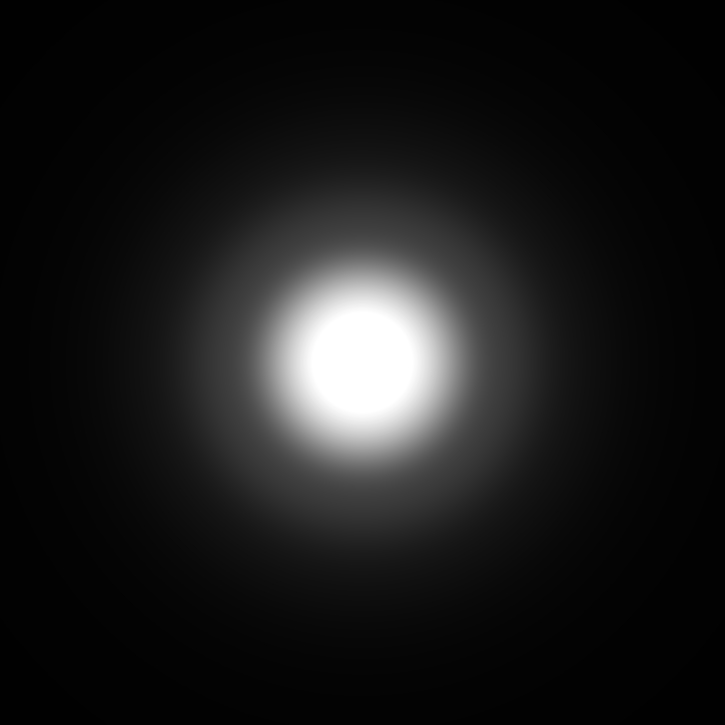
\includegraphics[height=\resLen]{slab/N1_300nm.jpg} &
        %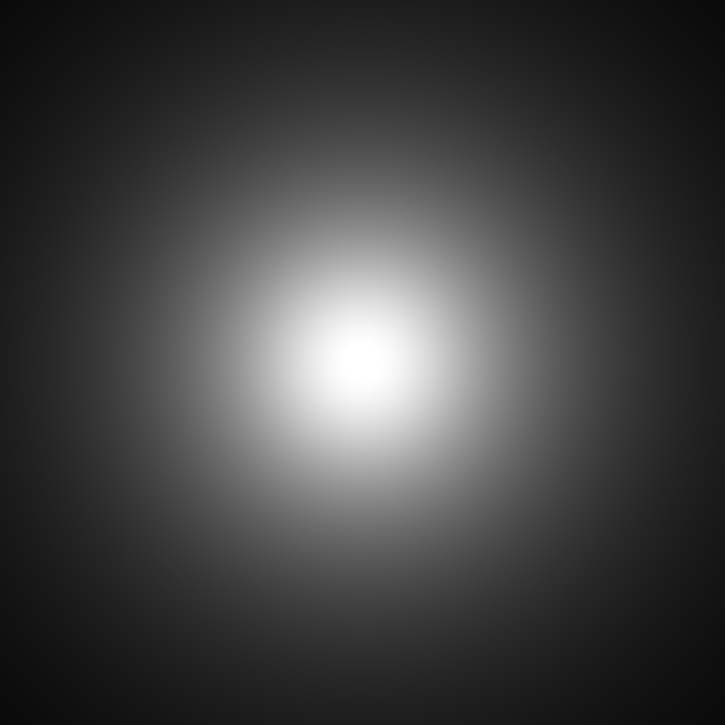
\includegraphics[height=\resLen]{slab/N1_500nm.jpg} &
        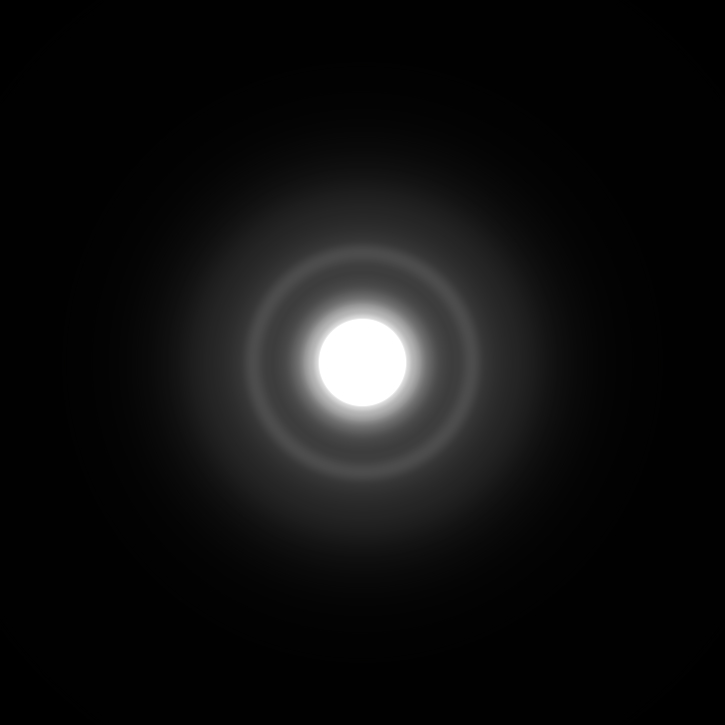
\includegraphics[height=\resLen]{slab/N100_300nm.jpg} &
        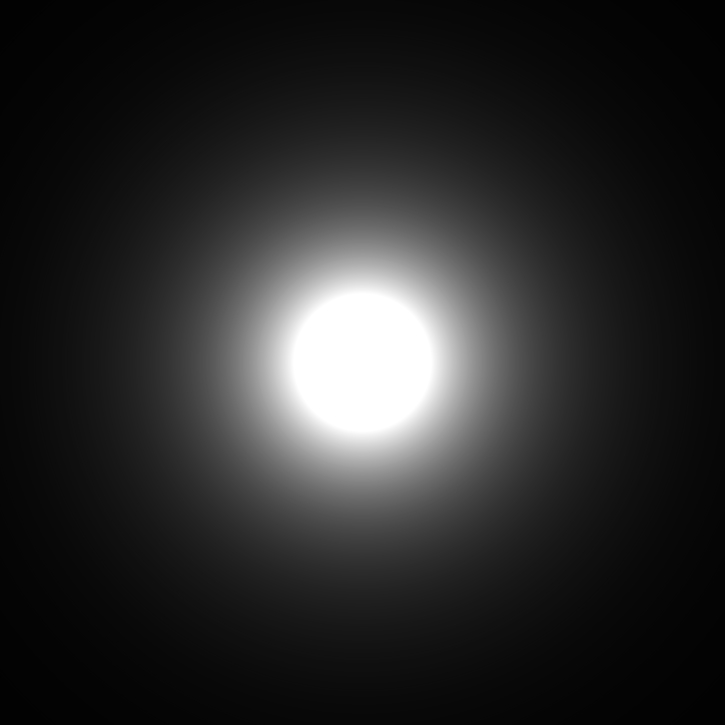
\includegraphics[height=\resLen]{slab/N100_500nm.jpg} &
        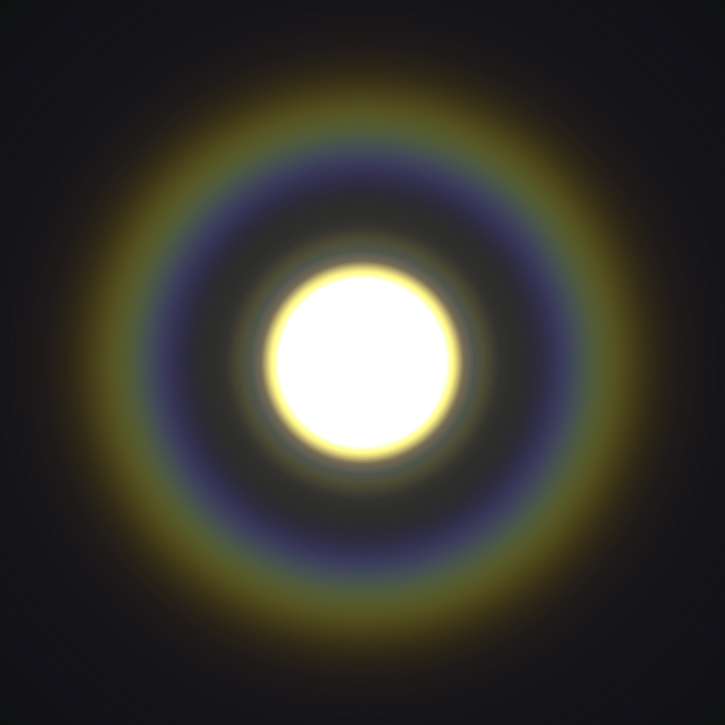
\includegraphics[height=\resLen]{slab/color.jpg} & 
        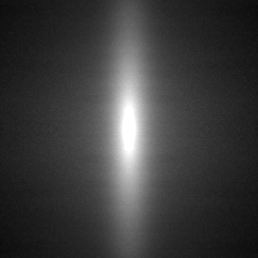
\includegraphics[height=\resLen]{slab/aniso_y.jpg} &
        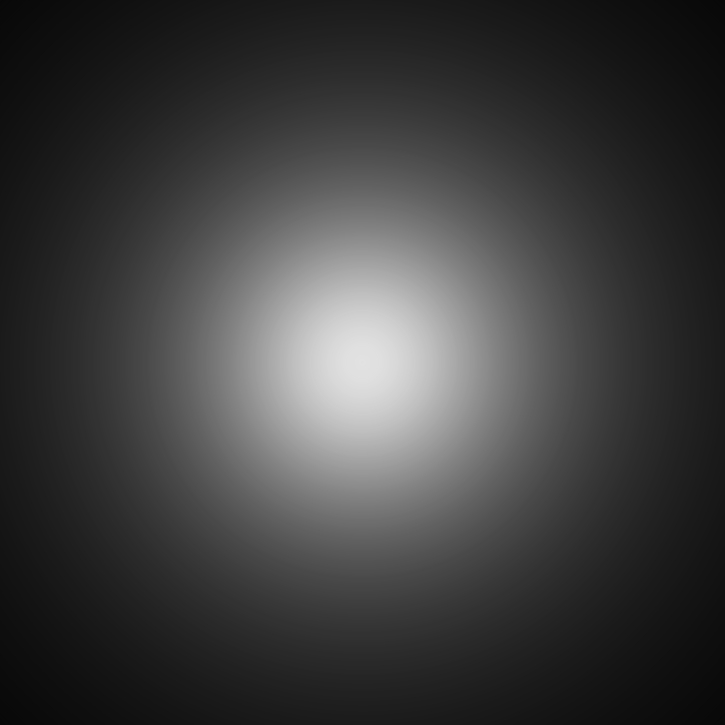
\includegraphics[height=\resLen]{slab/pos.jpg}
        \\
        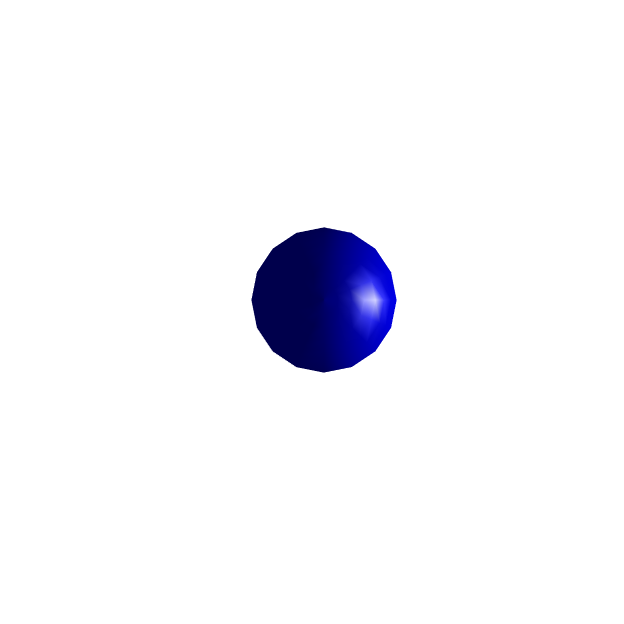
\includegraphics[height=\resLen]{particle/300nm_N1.png} &
        %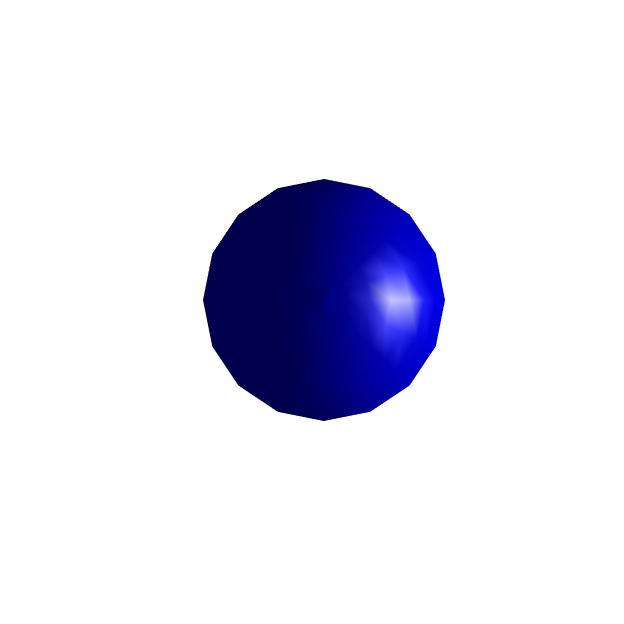
\includegraphics[height=\resLen]{particle/500nm_N1.png} &
        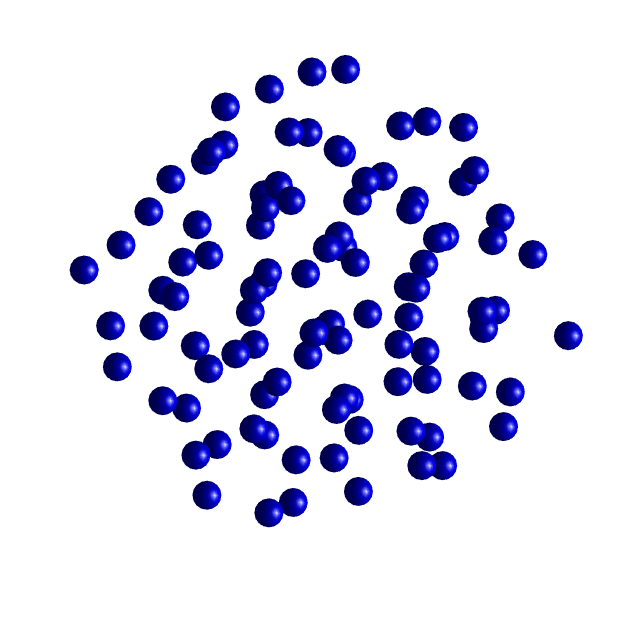
\includegraphics[height=\resLen]{particle/300nm_N100.png} &
        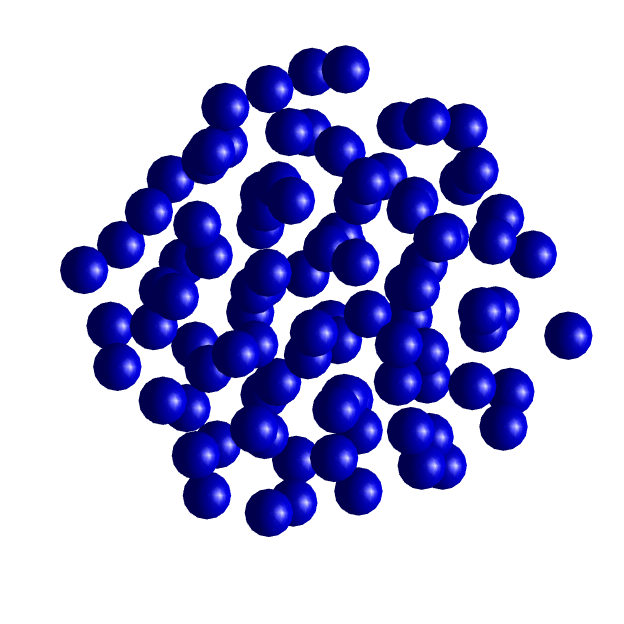
\includegraphics[height=\resLen]{particle/500nm_N100.png} &
        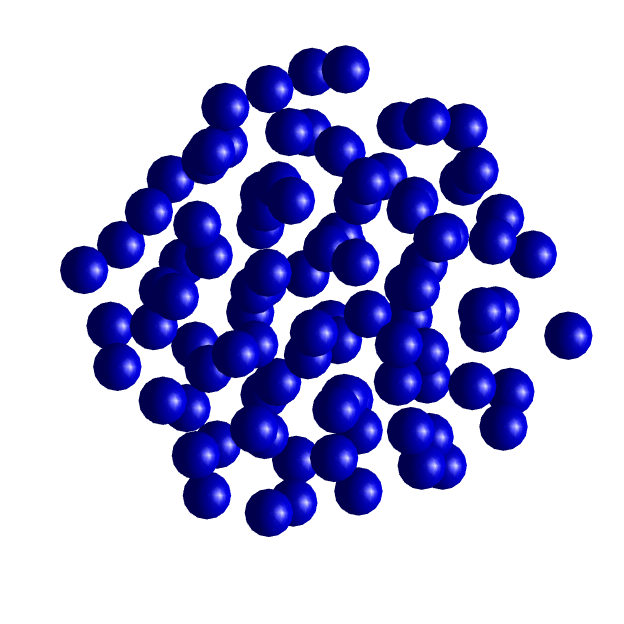
\includegraphics[height=\resLen]{particle/500nm_N100.png} &
        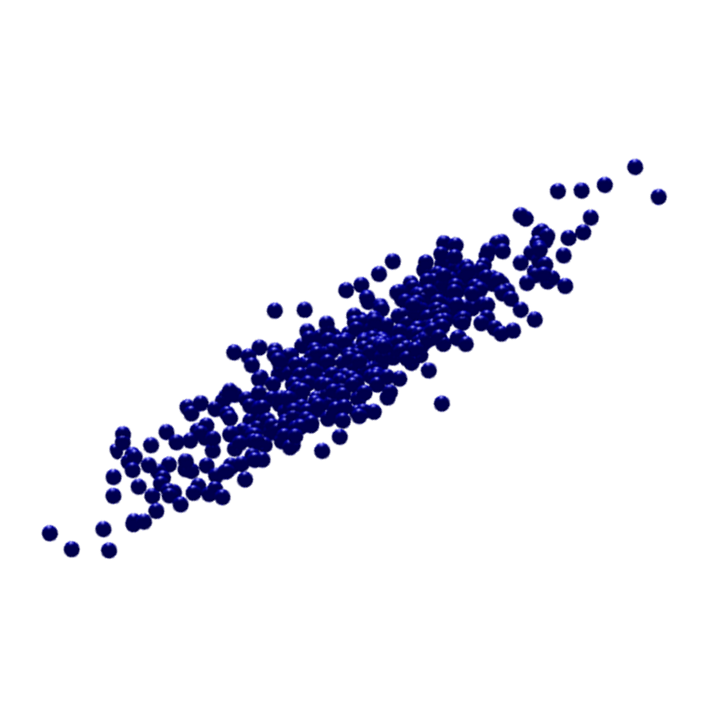
\includegraphics[height=\resLen]{particle/aniso.png} &
        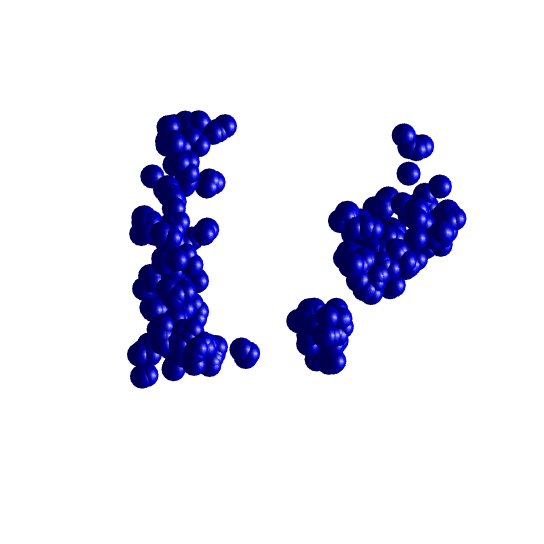
\includegraphics[height=\resLen]{particle/pos.png}
        \\
        $\Ncls=1$, $\radius_i=300\text{nm}$ &
        $\Ncls=100$, $\radius_i=300\text{nm}$ &
        $\Ncls=100$, $\radius_i=500\text{nm}$ &
        $\Ncls=100$, $\radius_i=500\text{nm}$ & 
        $\Ncls=100$, $\radius_i=500\text{nm}$ &
        $\Ncls=100$, $\radius_i=500\text{nm}$
        \\
        Isotropic & Isotropic & Isotropic & Isotropic & Anisotropic & Postively correlated
        \\
        $\lambda=700\text{nm}$ &
        $\lambda=700\text{nm}$ &
        $\lambda=700\text{nm}$ &
        Multi-spectral &
        $\lambda=700\text{nm}$ &
        $\lambda=400\text{nm}$
    \end{tabular}
    \caption{\label{fig:teaser}
        We introduce a new technique to compute bulk scattering parameters (i.e., the extinction and scattering coefficients as well as the single-scattering phase function) in a systematic fashion. By considering wave optical effects and particle (scatterer) interactions at the microscopic level, our technique enjoys the generality of supporting a wide range of media (e.g., isotropic, anisotropic, and correlated).
        In this figure, we show renderings of thin slabs lit with a small area light from behind (top).
        Additionally, we show visualizations of the corresponding particle distributions (middle) as well as per-cluster particle counts~$\Ncls$ radii $\radius_i$ (bottom).
    }
\end{teaserfigure}

    \maketitle
    %
    \section{Introduction}
\label{sec:intro}
%
Participating media and translucent materials---such as marble, milk, wax, and human skin---are ubiquitous in the real world. These materials allow light to penetrate their surfaces and scatter in the interior. 
%
In computational optics and computer graphics, how light interacts with participating media and translucent materials is typically modeled using the radiative transfer theory (RTT). Under this formulation, a participating medium consists of microscopic particles (\emph{scatterers}) randomly dispersed in some homogeneous embedding medium. After entering a translucent material, light travels in straight lines in the embedding medium and occasionally collides with a particle and gets redirected into a new direction. To capture the macroscopic behavior of light, the RTT uses a statistical description of the particles (the medium bulk parameters), namely the extinction coefficient $\sigT$ (aka. optical density), the scattering coefficient $\sigS$, and the phase function $\phase$.

While purely phenomenological in origin, the RTT has been demonstrated a corollary of Maxwell equations, under the assumption of far-field or independent scattering~\cite{mishchenko2002vector}. Therefore, these optical bulk parameters can be obtained from first principles, using e.g., Lorenz-Mie theory~\cite{hulst1981light,frisvad2007computing}. However, although very successful in practice, this theory neglects the interactions occurring between particles in their near-field, including wave-optics effects such as diffraction and interference with neighbor particles.  Consequently, Lorenz-Mie theory is largely limited to isotropic media with relatively low packing rates.  \rev{Examples of particles arranged as clusters---or falling in the near-field region of each other---are widespread in nature: From dense media where the particles density and packing rate is large, to spatially-correlated media such as clouds or biological structures where microscopic scatterers form clusters.}

Previously, the classical radiative transfer theory has been generalized to handle materials with (statistically) organized microstructures. 
Anisotropic media~\cite{jakob2010radiative}, for instance, have bulk scattering parameters with stronger directional dependency compared to isotropic media.
Additionally, media comprised of particles with correlated locations can exhibit non-exponential transmittance and characteristic scattering profiles~\cite{bitterli2018radiative,jarabo2018radiative}.
Although several empirical models have been proposed to model these media, \rev{these models work on the macro-scale directly, they are still based on the very same far-field assumption of Lorenz-Mie scattering, and lack the generality to capture wave-optics or multi-spectral effects.}Therefore, techniques capable of computing the bulk optical parameters of a material, based on its microscopic properties, have been lacking.

In this paper, we bridge this gap by introducing a new technique to systematically and rigorously compute the bulk scattering parameters. %for media formed by clusters of particles in their near-field region.
The elementary building block of our technique is \emph{particle clusters} in which individual particles follow user-specified distributions.
Within a cluster, we consider full near-field light transport effects; Between clusters, on the contrary, we use a far-field approximation to allow efficient modeling of macroscopic level light transport.

Our formulation is derived from first principles of light transport (i.e., Maxwell electromagnetism) and reduces to the Lorenz-Mie theory in the special case of single-particle scatterers. Based on this formulation, we demonstrate how the bulk parameters can be computed numerically. Using our technique, we systematically generate radiative transfer optical parameters capturing multi-spectral, anisotropic, and correlated scattering effects for particles with arbitrary distributions (Figure~\ref{fig:teaser}).

Concretely, our contributions include:
%
\begin{itemize}
    \item Establishing a computational framework for modeling light scattering from clusters of particles (\S\ref{sec:ours_theory}).
    %
    \item Showing how radiative transfer parameters can be computed numerically based on our formulation (\S\ref{sec:ours_numerical}).
    %
    \item Demonstrating how our technique can be applied to systematically compute scattering parameters for a variety of participating media (\S\ref{sec:result}).
\end{itemize}

    \section{Related Work}
\label{sec:prior}
%
\paragraph{Radiative transfer. } 
Simulating the propagation of light in participating media has been widely studied in graphics~\cite{novak2018monte}, building upon the radiative transfer equation (RTE), introduced 125 years ago by von Lommel~\shortcite{lommel1889photometrie} (see \cite{mishchenko2013125} for a historical perspective). 
%
This scalar radiative formulation has been extended in graphics accounting for anisotropic~\cite{jakob2010radiative}, refractive~\cite{ament2014refractive}, bispectral~\cite{gutierrez2008visualizing}, or spatially-correlated media~\cite{jarabo2018radiative,bitterli2018radiative}. All these works assume a radiometric light transport model, establishing no connections with the electromagnetic behaviour governing light transport. 
%
From a wave-optics perspective, a few works have generalized light transport in media to account for wave-based properties, including polarized light transport~\cite{wilkie2001combined,Jarabo2018bidirectional}, or coherence~\cite{bar2019monte}. This last work is of special relevance, given that it was able to simulate purely wave-based phenomena such as speckle or coherent back-scattering on top of a radiative model. 
%
All these works build on the assumption of the far-field approximation and independent scattering, which largely simplifies computations. A notable exception is the near-field model proposed by Bar et al.~\shortcite{bar2020rendering}, that renders speckle statistics in the near-field zone of the camera, although it still considers independent far-field scattering between particles. In contrast, in this work we explicitly relate the radiometric light transport modeled by the RTE with physics-based optics based on electromagnetism, and generalize the independent scattering approximation to account clusters of particles in the near field. 


\paragraph{Modeling scattering in media}
%
The phase function models the average scattering distribution at a light interaction with the medium. A common approach is to use simple phenomenological models, such as the Henyey-Greenstein phase function~\cite{henyey1941diffuse} or mixtures of von Mishes-Fisher distributions~\cite{gkioulekas2013understanding}, as well as other functions modeling the scattering of idealized anistropic particles~\cite{zhao2011building,heitz2015sggx}; however, these methods lack an explicit relationship with the underlying microscopic material properties. Under the assumption of geometric optics, several works have proposed to precompute the phase functions of more complex particles for granular materials~\cite{meng2015multi,muller2016efficient} or cloth fibers~\cite{aliaga2017appearance} using explicit path tracing, by neglecting wave effects. 
%
A more rigorous phase function is based on the Lorenz-Mie theory~\cite{hulst1981light}, which provides closed-form solutions for the Maxwell's equations for spherical particles~\cite{jackel1997modeling,frisvad2007computing}. Sadeghi et al.~\shortcite{sadeghi2012physically} generalized the Lorenz-Mie theory to larger non-spherical particles in the context of accurately modeling rainbows. To avoid the expensive sum series of the Lorenz-Mie theory, Guo et al.~\shortcite{guo2021rendering} proposed to use the geometric optics approximation~\cite{glantschnig1981light}, which gives a good approximation to Lorenz-Mie theory for larger particles at significantly lower cost. 
%
All these approaches provide accurate rigorous solutions to the far-field scattering of disperse particles. 

Beyond Lorenz-Mie, several exact rigorous solutions have been proposed for computing  electromagnetic scattering of particles in media, including the finite elements method (FEM), the finite difference time domain (FDTD) method, or the boundary elements method (BEM)~\cite{wu1977scattering}, which solve the Maxwell's equations for arbitrary shapes. Xia et al.~\shortcite{xia2020wave} proposed using BEM for accurately precomputing the far-field scattering of individual fibers. Unfortunately these methods are very slow as the number of particles increases, limiting its applicability to individual elements in problems with reduced dimensionality. 
%
The T-matrix method~\cite{waterman1965matrix} generalizes the Lorentz-Mie theory to particles of arbitrary shape in both the near- and far-fields, with the only assumption of the computed field being outside a sphere surrounding the particles. This method was later extended to clusters of multiple particles~\cite{peterson1973t,mackowski2011multiple}. We leverage the T-matrix method for computing the scattering of groups of particles. 

\paragraph{Wave optics in surface scattering} 
Inspired on the vast background on electromagnetic surface scattering in optics (see \cite{frisvad2020survey} for a general survey), several works in graphics have taken into account relevant wave effects including diffraction-aware BSDFs~\cite{he1991comprehensive,Stam:1999:DiffractionShaders,Cuypers:2012:Diffraction,dong2015predicting,Holzschuch:2017:Two, Toisoul:2017:practical, Werner:2017:ScratchIridescence,Yan:2018:WavesMicrogeometry},  goniochromatic patterns due to thin-layer interference~\cite{Smits:1992:Newton,Gondek:1994:WavelengthDependent,Belcour:2017:Iridescence,guillen2020general}, or birefringence~\cite{Steinberg:2019:Analytic}. These works assume single scattering, with no interaction between different particles with a few exceptions that assume full incoherence after single scattering~\cite{Falster:2020:Computing,guillen2020general}. Notably, Moravec~\shortcite{moravec19813d} and Musbach et al.~\shortcite{musbach2013full} computed the full electromagnetic surface scattering by solving the wave propagation using the FDTD method. 
%

    \section{Preliminaries}
\label{sec:prelim}
%
We now briefly revisit the basics on first principles of (classical) light transport theory based on Maxwell electromagnetism. Table~\ref{tb:symbols} summarizes the symbols used along the paper.
\begin{table}[t]
    \caption{Symbols used along the paper.}
    \label{tb:symbols}
    \footnotesize
    %
    \addtolength{\tabcolsep}{-1pt}
    \renewcommand{\arraystretch}{1.1}
    \begin{tabular}{cl}
        \textbf{Symbol}   & \textbf{Definition} \\ 
        \toprule
        $\px\in\Real^3$ & Position \\
        $\dpx\in\Sphere$ & Direction to $\px$ \\
        $\tpx\in\Real$ & Distance \\
        \hline
        $\sPermittivity(\px)$ & Permittivity \\
        $\sPermeability(\px)$ & Permeability \\
        $\sFreq$ & Wave angular frequency [s$^{-1}$] \\
        $\lambda=2\pi\sFreq^{-1}$ & Wavelength [m] \\
        $k(\px)=\sFreq\sqrt{\sPermittivity(\px)\sPermeability(\px)}$ & Wavenumber at $\px$\\
        $\sIOR(\px)=k_2(\px)/k_1$ & Relative refractive index at $\px$ \\
        \hline
        $\MField(\px)$ & Magnetic field at $\px$ \\
        $\EField(\px)$   & Electric field at $\px$~\eqref{eq:vri}  \\
        $\IncEField(\px)$ & Incident electric field $\px$\\
        $\ScaEField(\px)$ & Scattered electric field at $\px$~\eqref{eq:vri}\\ 
        $\EField_0$ & Amplitude of a planar electric field \\
        $\ScaEField_1(\dpx)$ & Far-field angular distribution of the scattered radiation  \\
        \hline
        $\sGreen$ & Free-space dyadic Green's function~\eqref{eq:greenfunc} \\
        $\dyad{T}$ & Dyad transition operator~\eqref{eq:dyadtransition}\\
        $\sGreenProp(\dw,\px)$ & Planar field scalar propagator \\
        \hline
        \hline
        $V_i$ & Volume suspended by particle/cluster $i$ \\
        $\Px_i\in\Real^3$ & Representative position of particle/cluster $i$ \\
        $\dPx_{ij}\in\Sphere$ & Direction from $\Px_j$ to $\Px_i$\\
        $\tPx_{ij}\in\Real$ & Distance from $\Px_j$ to $\Px_i$\\
        $\Ncls$ & Number of particles in a cluster \\
        \hline
        $\ScaEField_i(\px)$ & Scattered field of $\px\in V_i$~\eqref{eq:foldylax}\\
        $\EField_i(\px)$ & Exciting field in $\px\in V_i$ \\
        $\ExcEField_{ij}(\px)$ & Partial exciting field in $\px\in V_i$ from particle $j$~\eqref{eq:excfield} \\
        $\ScaDyad_i^\text{near}(\dwi,\px)$ & Near-field scattering dyad of particle/cluster $i$~\eqref{eq:scatdyad_near} \\
        $\ScaDyad_i(\dwi,\dws)$ & Far-field scattering dyad of particle/cluster $i$~\eqref{eq:farscatdyad} \\
        \hline
        \hline
        $\cT(\dwi),\cS(\dwi)$ & Extinction~\eqref{eq:crosstcluster} and scattering~\eqref{eq:crossscluster} cross-sections [m$^{2}$]\\
        $\phase(\dwi,\dws)$ & Phase function~\eqref{eq:phasecluster} [sr$^{-1}$]\\
        $\rho$ & Particles density [m$^{-3}$] \\
        $\sigT(\dwi),\sigS(\dwi)$ & Extinction~\eqref{eq:sigmatcluster} and scattering~\eqref{eq:sigmascluster} coefficients [m$^{-1}$]\\
        \bottomrule
    \end{tabular}
\end{table}

\subsection{Electromagnetic Scattering}
\label{ssec:prelim_maxwells}
%
The propagation of a time-harmonic monochromatic electromagnetic field with frequency $\sFreq$ is defined by the Maxwell curl equations as
\begin{equation}
    \begin{aligned}
        \Curl\EField(\px) &= \img\,\sFreq\,\sPermeability(\px)\,\MField(\px),\\
        \Curl\MField(\px) &= -\img\,\sFreq\,\sPermittivity(\px)\,\EField(\px),
    \end{aligned}
    \label{eq:maxwell}
\end{equation}
%
where $\Curl.$ is the curl operator; $\EField(\px)$ and $\MField(\px)$ indicate, respectively, the (vector-valued) electric and magnetic fields at $\px$; $\sPermeability(\px)$ and $\sPermittivity(\px)$ denote the (scalar-valued) magnetic permeability and electric permittivity at $\px$, respectively; and $\img := \sqrt{-1}$ is the imaginary unit.

Assuming a non-magnetic medium satisfying $\sPermeability(\px) = \sPermeability_0$ with $\sPermeability_0$ being the magnetic permeability of a vacuum, \Eq{eq:maxwell} reduces to the electric field wave equation
%
\begin{equation}
    \nabla^2\times\EField(\px) - k(\px)^2\,\EField(\px) = 0,
    \label{eq:efieldwave}
\end{equation}
%
where \rev{$\nabla^2=\Curl\nabla$}, and $k(\px) = \sFreq\sqrt{\sPermittivity(\px)\sPermeability_0}$ is the medium's wave number at $\px$. \rev{Note that the wave number $k$ has a dependence on the frequency $\sFreq$; in the following we omit such dependence for brevity.}

We now assume an infinite homogeneous isotropic medium with permittivity $\sPermittivity_1$, filled with scatterers bounded by a finite disjoint region $V$, with potentially inhomogeneous permittivity $\sPermittivity_2(\px)$. Under this assumption, we can solve \Eq{eq:efieldwave} by expressing it as the \emph{volume integral equation} (see \S S1 on the supplemental or \S 3.1 of Mishchenko's work~\shortcite{mishchenko2006multiple} for a step-by-step derivation) as the sum of the incident field $\IncEField(\px)$ and the scattered field $\ScaEField(\px)$ due to inhomogeneities in the medium in the form of scatterers:
%
\begin{align}
    \EField(\px) & = \IncEField(\px) + \ScaEField(\px) \\
    & =\IncEField(\px) + k_1^2\,\int_V [\sIOR^2(\px')-1] \,\sGreen(\px,\px') \cdot \EField(\px') \diff{\px'},
    \label{eq:vri}
\end{align}
%
with $k_1$ the wave number at the hosting medium, $\sIOR(\px) = \nicefrac{k_2(\px)}{k_1}$ the index of refraction of the interior regions $V$ with respect to the hosting medium, \rev{the operator $.\cdot.$ is the dot product\footnote{In the paper we use $.\cdot.$ as the vector-vector, vector-dyadic and dyadic-dyadic dot products.}} and $\sGreen(\px,\px')$ the free-space dyadic Green's function defined as:
%
\begin{equation}
    \sGreen(\px,\px') = \left(\sIdDyad + k_1^{-2}\,\nabla\otimes\nabla\right) \frac{\exp(\img\,k_1 \,|\px-\px'|)}{4\pi\,|\px-\px'|},
    \label{eq:greenfunc}
\end{equation}
%
where $\sIdDyad$ is the identity dyad, and $. \otimes .$ denotes the dyadic product of two vectors. \rev{Note that the derivative operator $\nabla$ applies over $\px$.} Intuitively, \Eq{eq:vri} models the scattering field as the superposition of the spherical wavelets resulting from a change of permittivity (i.e. with $\sIOR(\px')\neq1$). Note also the recursive nature of \Eq{eq:vri}; we will deal with this recursivity in the following section, computing $\ScaEField(\px)$ as a function of the incident field $\IncEField(\px)$. 

\begin{figure*}
\centering
  \def\svgwidth{.5\columnwidth}
  \input{img/scheme/fig1.pdf_tex} \qquad
  \def\svgwidth{.7\columnwidth}
  \input{img/scheme/fig2.pdf_tex} \qquad
  \def\svgwidth{.6\columnwidth}
  \input{img/scheme/fig3.pdf_tex}
  
  \caption{Schematical representation of the particles scattering geometry. Previous methods, including Lorenz-Mie theory, assume independent scattering of particles (left), assuming that the distance $\tPx_{ij}$ between two particles $i$ and $j$ is very large (i.e., $\tPx_{ij}\rightarrow\infty$), neglecting the potential interactions between particles. In our work (middle) we differentiate between near field scattering of particles within a small region in space (cluster $\Cls$ centered at $\Px_\Cls$), and particles $k$ on the far-field region of the cluster (distance $\tPx_{\Cls k}\rightarrow\infty$). For large values of $\tPx_{\Cls k}$, the direction between particle $k$ and any particle $j\in\Cls$ is $dPx_{ik}\approx\dPx_{\Cls k}$: Therefore, we can assume a planar exciting field $\ExcEField_{\Cls k}(\px)$ on the whole cluster $\Cls$ from particle $k$, with direction $\dPx_{\Cls k}$ (right). }
\label{fig:diagram}
\end{figure*}

\subsection{Foldy-Lax Equations}
\label{ssec:foldy-lax}
%
We now consider a medium filled with $N$ finite discrete particles with volume $V_i$ and index of refraction $\sIOR_i(\px)$. Considering an incident E-field $\IncEField(\px)$, we can rewrite \Eq{eq:vri} as
%
\begin{equation}
    \EField(\px) = \IncEField(\px) + \int_{\Real^3} U(\px')\,\sGreen(\px,\px') \cdot \EField(\px') \diff{\px'},
    \label{eq:EfieldParticles}
\end{equation}
%
where $\sGreen(\px,\px')$ is the dyadic Green's function~\eqref{eq:greenfunc}, and $U(\px)$ the potential function given by
%
\begin{equation}
    U(\px) = \sum_{i=1}^{N} U_i(\px) \quad \text{with} \quad U_i(\px) = \begin{cases} 
    0, & (\px \notin V_i)\\ 
    k_1^2[\sIOR_i^2(\px)-1]. & (\px \in V_i)
    \end{cases}
    \label{eq:potential}
\end{equation}
%
By combining \Eqs{eq:EfieldParticles}{eq:potential}, we can express the field at any position $\px\in\Real^3$ following the so-called \emph{Foldy-Lax equation}~\cite{foldy1945multiple,lax1951multiple} as
%
\begin{equation}
\EField(\px) = \IncEField(\px) + \sum_{i=1}^N \overbrace{\int_{V_i} \sGreen(\px,\px') \cdot \int_{V_i} \dyad{T}_i(\px',\px'') \cdot \EField_i(\px'') \diff{\px''}\,\diff{\px'}}^{\eqdef \,\ScaEField_i(\px)},    \label{eq:foldylax}
\end{equation}
%
with $\ScaEField_i(\px)$ and $\EField_i(\px)$ the scattered and partial field of particle $i$, and $\dyad{T}_i(\px,\px')$ the dyad transition operator for particle $i$ defined as~\cite{tsang1985theory} 
\begin{equation}
\label{eq:dyadtransition}
    \begin{split}
        \dyad{T}_i(\px,\px') =\;& U_i(\px) \,\delta(\px-\px')\,\sIdDyad \\
        & + U_i(\px) \int_{V_i} \sGreen(\px,\px'') \cdot \dyad{T}_i(\px'',\px') \diff{\px''},
    \end{split}
\end{equation}
%
with $\delta(x)$ the Dirac delta. 
%
The partial field at particle $i$ is defined as $\EField_i(\px)=\IncEField(\px) + \sum_{j(\neq i)=1}^N \ExcEField_{ij}(\px)$, where the partial exciting field $\ExcEField_{ij}(\px)$ from particles $j$ to $i$ is 
\begin{equation}
\ExcEField_{ij}(\px) = \int_{V_j} \sGreen(\px,\px')\cdot\int_{V_j} \dyad{T}_j(\px',\px'')\cdot \EField_j(\px'') \diff{\px''}\,\diff{\px'},
\label{eq:excfield}
\end{equation}
%
with $\px\in V_i$. Note that the scattered and exciting fields for particle $j$ have essentially the same form. 
%
As shown by Mishchenko \shortcite{mishchenko2002vector}, the Foldy-Lax equation~\eqref{eq:foldylax} solves exactly the volume integral equation~\eqref{eq:vri} for multiple arbitrary particles in the medium, without any assumptions on their composition or packing rate, beyond the assumption of a homogeneous hosting medium.

%\sz{Maybe also review the Mie theory (by talking about what it solved under this formulation. Also, need to describe how the key equations are used by us (e.g., what is being solved by our simulations).}

\paragraph{Far-field Foldy-Lax Equations}
\Eq{eq:excfield} defines the exact exciting field resulting from the scattering by particle~$j$ on particle~$i$.
However, if the distance $\tPx_{ij} \defeq \| \Px_i - \Px_j \|$ between particles (with $\Px_i$ denoting the center of particle $i$) is large, we can approximate the propagation distance between any point $\px \in V_i$ and $\px' \in V_j$ as
%
\begin{equation}
    \| \px - \px' \| \approx \tPx_{ij} + (\dPx_{ij} \cdot {\Delta}\px) -  (\dPx_{ij} \cdot {\Delta}\px'),
\end{equation}
%
with $\dPx_{ij} \defeq \nicefrac{(\Px_i - \Px_j)}{\tPx_{ij}}$, ${\Delta}\px \defeq \px - \Px_i$ and ${\Delta}\px' \defeq \px' - \Px_j$ (see Figure~\ref{fig:diagram}, left).
%With this approximation, we can now express $\ExcEField_{ij}(\px)$ for a point $\px \in V_i$ using its \emph{far-field} approximation, as:%
%\footnote{We note that, accordingly to Mishchenko~\shortcite{mishchenko2006multiple}, the product would require to multiply the integrand by the dyad $(\sIdDyad - \dPx_{ij}\otimes\dPx_{ij})$ to ensure a transverse planar field; we remove it for clarity.}
%
%\begin{equation}
%    \begin{split}
%        & \ExcEField_{ij}(\px)\\
%        \approx\;& \frac{\E^{\img k_1 (\tPx_{ij}+\dPx_{ij}\cdot{\Delta}\px)}}{4\pi\tPx_{ij}} \int_{V_j} \sGreenProp(\dPx_{ij},{\Delta}\px') \int_{V_j} \dyad{T}_j(\px',\px'')\cdot \EField_j(\px'') \diff{\px''}\,\diff{\px'} \\
%        =\;& \frac{\exp(\img k_1 \,\tPx_{ij})}{\tPx_{ij}} 
%        \sGreenProp(\dPx_{ij}, \Delta \px) \,\ExcEField_{1ij}(\dPx_{ij}),
%    \end{split}
%    \label{eq:excfieldfar}
%    \raisetag{17pt}
%\end{equation}
%
%where: $\px \in V_i$ is a point in particle $i$; $\sGreenProp(\dw, \Delta \px)=\exp(\img k_1 \,\dPx_{ij}\cdot{\Delta}\px)$; and $\ExcEField_{1ij}$ is the far-field exciting field from particle $j$ to particle $i$ that is solely characterized by the propagation direction $\dPx_{ij}$. 
\rev{
With this approximation, we can now express $\ExcEField_{ij}(\px)$ for a point $\px\in V_i$ using its \emph{far-field} approximation (see \S{S3} in the supplemental for the derivation), as%\footnote{Note that accordingly to Mishchenko~\shortcite{mishchenko2002vector} the product would require to multiply the integrand by the dyad $(\sIdDyad - \dPx_{ij}\otimes\dPx_{ij})$ to ensure a transverse planar field; we remove it for clarity.}:
%
\begin{equation}
\label{eq:excfieldfar}
\ExcEField_{ij}(\px) = \frac{\exp(\img k_1 \,\tPx_{ij})}{\tPx_{ij}} \sGreenProp(\dPx_{ij}, \Delta \px) \,\ExcEField_{1ij}(\dPx_{ij}),
\end{equation}
%
with $\px\in V_i$ a point in particle $i$, $\sGreenProp(\dw,\px)=\exp(\img k_1 \dw\cdot \px)$, and $\ExcEField_{1ij}$ the far-field exciting field from particle $j$ to particle $i$ defined as
%
\begin{align}
    \ExcEField_{1ij}(\dPx_{ij}) & = (4\pi)^{-1}(\sIdDyad - \dPx_{ij}\otimes\dPx_{ij})\\ & \cdot \int_{V_j} g(-\dPx_{ij}, {\Delta}\px') \int_{V_j} \dyad{T}_j(\px',\px'') \cdot \EField_j(\px'') \diff{\px''}\diff{\px'} \nonumber.
\end{align} 
The dyad $(\sIdDyad - \dPx_{ij}\otimes\dPx_{ij})$ ensures a transverse planar field, which allows to solely characterize $\ExcEField_{1ij}(\dPx_{ij})$ by the propagation direction $\dPx_{ij}$.}In order for \Eq{eq:excfieldfar} to be valid, the distance $\tPx_{ij}$ needs to hold the far-field criteria, which relates the $\tPx_{ij}$ with the radius of the particle $\radius_j$ following the inequality~\cite{mishchenko2006multiple}:
%
\begin{equation}
    k_1 \tPx_{ij} \gg \max\left(1, \frac{k_1^2\radius_j^2}{2}\right).
    \label{eq:farfield}
\end{equation}
%
%The Lorenz-Mie theory~\cite{hulst1981light} builds upon this far-field assumption to model electromagnetic scattering from small (spherical) particles which as shown by Mishchenko~\shortcite{mishchenko2002vector} is at the core assumptions of radiative transfer theory. 
This far-field assumption is both the basis for the Lorenz-Mie theory~\cite{hulst1981light} (to model electromagnetic scattering from small spherical particles) and, as shown by Mishchenko~\shortcite{mishchenko2002vector}, at the core of the radiative transfer theory.

In the following, we relax the assumption of near-field scattering and compute the Foldy-Lax equations for clusters of particles for both the near- and far-field regions. Then, we use them to compute the scattering matrix to be used in the RTE to efficiently approximate light transport between clusters of particles. 




% \gy{------------ updated -------------}
% \begin{equation}
%         \nabla\cdot\EField(\px) = 0
%     \label{eq:maxwell_update1-1}
% \end{equation}
% \begin{equation}
%         \nabla\cdot\MField(\px) = 0
%     \label{eq:maxwell_update1-2}
% \end{equation}
% \begin{equation}
%         \Curl\EField(\px) = \img\,\sFreq\,\sPermeability(\px)\,\MField(\px)
%     \label{eq:maxwell_update1-3}
% \end{equation}
% \begin{equation}
%         \Curl\MField(\px) = - \img\,\sFreq\,\sPermittivity(\px)\,\EField(\px)
%     \label{eq:maxwell_update1-4}
% \end{equation}

% Take the curl of both sides of (\ref{eq:maxwell_update1-3}) and together with (\ref{eq:maxwell_update1-4}),
% \begin{equation}
%         \Curl(\Curl\EField(\px)) = \img\,\sFreq\,\sPermeability(\px)\,(\Curl\MField(\px)) =
%         \sFreq^2\,\sPermeability(\px)\,\sPermittivity(\px)\,\EField(\px)
% \end{equation}

% Using vector identity
% \begin{equation}
%     \nabla\times(\nabla\times\mathbf{E}) = \nabla(\nabla\cdot\mathbf{E}) - \nabla\cdot(\nabla\mathbf{E}) = - \nabla\cdot(\nabla\mathbf{E}) = -\nabla^2\mathbf{E} \label{CurlOfCurl}
% \end{equation}

% equation (\ref{eq:maxwell_update1-3}) reduce to
% \begin{equation}
%     \nabla^2\EField(\px) + k^2\,\EField(\px) = 0
%     \label{eq:efieldwave_update}
% \end{equation}

% \gy{------------ updated -------------}
    \section{Scattering from Clusters of Particles}
\label{sec:ours_theory}
%
%\sz{We should add a table of symbols with ``links'' to their definitions.}
%
In this section, we present our main theoretical result: the far-field approximated scattering dyad relating a field incoming at a particle, which will be shown in \Eq{eq:farscatdyad}.
This dyad can then be used to compute a medium's bulk scattering parameters, which we will discuss in \S\ref{ssec:ours_RTT}.

The two forms of computing the exciting field from particle $j$ to $i$ [\Eqs{eq:excfield}{eq:excfieldfar}] suggest that we can consider two subsets of particles $j$ depending on their distance with respect to the point of interest $\px$: One set of $\Nnear$ particles in the near field and another set of $\Nfar$ particles in the far field. With that, we can now calculate the exciting field in particle $i$ as:
%
\begin{equation}
    \EField_i(\px)= \IncEField(\px) + \sum_{j(\neq i)=1}^\Nnear \ExcEField_{ij}(\px) + \sum_{k=1}^\Nfar \ExcEField_{ik}(\px).
    \label{eq:foldylaxtwo}
\end{equation}

In what follows, we derive the far-field Foldy-Lax equations for groups of particles where a cluster of these particles are in their respective near-field region, while the other elements in the system are in the far field. For the simplicity of our derivations, we consider a single far-field incident field in the cluster, and assume that the far-field particles $k$ do not have neighbor particles in their respective near field region.
%
More formally, we now consider a cluster $\Cls$ of $N_\Cls$ particles, where all particles $i\in\Cls$ are in their respective near-field region, and that the particles of the cluster have a bounding sphere centered at $\Px_\Cls$ with radius $\radius_\Cls$ (see Figure~\ref{fig:diagram}, middle). 

Since both the incident field $\IncEField(\px)$ and the exciting field $\ExcEField_{\Cls k}(\px)$ from particle $k$ are in the far-field region, we can assume both fields to be planar waves defined as
%
\begin{align}
    \label{eq:farincfieldcluster}
    \IncEField(\px) &= \IncEField_0 \,\exp(\img k_1 \dw \cdot \Delta \px) = \IncEField_0\,\sGreenProp(\dw, \Delta \px) , \\
    \ExcEField_{\Cls k}(\px) &= \ExcEField_{0\Cls k}\,\exp(\img k_1 \dPx_{\Cls k} \cdot \Delta \px) =  \ExcEField_{0\Cls k}\,\sGreenProp(\dPx_{\Cls k}, \Delta \px), 
    \label{eq:farexcfieldcluster} 
\end{align}
%  
with $\IncEField_0$ the amplitude of the planar incident field, $\dw$ its direction, and $\Delta \px=\px-\Px_\Cls$. Equivalently, $\ExcEField_{0\Cls k}=\frac{\exp(\img k_1 \,\tPx_{\Cls k})}{\tPx_{\Cls k}}\,\ExcEField_{1\Cls k}(\dPx_{\Cls k})$  is the amplitude of the exciting field at $\Cls$ from particle $k$, and $\dPx_{\Cls k}$ its direction. 

Now, let us slightly abuse the dot product notation, remove the dependency on the spatial dependency on each term, and use $(\varphi_1 \cdot \varphi_2) = \int \varphi_1(x)\,\varphi_2(x) \diff x$ for scalar-valued functions $\varphi_1$ and $\varphi_2$. From the far-field assumptions, plugging \Eq{eq:foldylaxtwo} into the definition of the scattered field from particle $i\in\Cls$ in Equation~\eqref{eq:foldylax} (with $\Nnear=\Ncls$) yields
%
\begin{equation}
    \label{eq:scafieldcluster1}
    \begin{split}
        \ScaEField_i(\px) &= \sGreen \cdot \dyad{T}_i\cdot \EField_i\\
        & = \sGreen \cdot \dyad{T}_i \cdot \left[\IncEField + \sum_{k=1}^\Nfar \ExcEField_{\Cls k}+ \sum_{j(\neq i)=1}^\Ncls \ExcEField_{ij} \right].
    \end{split}        
\end{equation}
%
By recursively expanding $\ExcEField_{ij}$ and some algebraic operations (see the supplemental for the full derivation), this results into 
\begin{align}
    \label{eq:scafieldcluster5}
    \ScaEField_i(\px) &= \EField_0 \, \sGreen \cdot \dyad{T}_i \cdot \Bigg[ \sGreenProp(\dw) + \sum_{j(\neq i)=1}^\Ncls \left[...\right]_j^{\sGreenProp(\dw)} \Bigg] \\
    & + \sum_{k=1}^\Nfar \ExcEField_{0\Cls j}\,\left[ \sGreen \cdot \dyad{T}_i \cdot \Bigg[ \sGreenProp(\dPx_{\Cls k}) + \sum_{j(\neq i)=1}^\Ncls \left[...\right]_j^{\sGreenProp(\dPx_{\Cls k})}\Bigg]\right]. \nonumber 
\end{align}
%
where the "$[...]_l^\varphi$" term represents the recursivity as
%
\begin{equation}
    [...]_j^\varphi= \sGreen \cdot \dyad{T}_j \cdot \left[\varphi + \sum_{l(\neq j)=1}^\Ncls \left[...\right]_l^\varphi\right] \,.
\end{equation}
%
Note that each element in the sum in \Eq{eq:scafieldcluster5} above is the result of the amplitude of the far-field incident or exciting fields, and a series that encode all the near-field scattering in the cluster $\Cls$. We can thus define the scattering dyad $\ScaDyad_i^\text{near}(\dwi,\px)$ relating a unit-amplitude planar incident field at particle $i$ from direction $\dwi$ with the scattered field at point $\px$ as
%
\begin{equation}
    \ScaDyad_i^\text{near}(\dwi,\px) = \sGreen \cdot \dyad{T}_i\cdot \Bigg[ \sGreenProp(\dwi) + \sum_{j(\neq i)=1}^\Ncls \left[...\right]_j^{\sGreenProp(\dwi)} \Bigg].
    \label{eq:scatdyad_near}
\end{equation}
%
By considering constant $\IncEField_0$ and $\ExcEField_{0\Cls k}$ for the whole cluster $\Cls$, we can compute the cluster's scattering dyad as:
%
\begin{equation}
    \ScaDyad_\Cls^\text{near}(\dwi,\px) = \sum_{i=1}^{N_\Cls} \ScaDyad_i(\dwi,\px),
    \label{eq:scatdyadcluster_near}
\end{equation}
%
%The scattering dyad $\ScaDyad_\Cls^\text{near}(\dwi,\px)$ solves
which defines the scattered field for a unit-amplitude incoming planar field in a scene consisting of the particles forming cluster $\Cls$.
In practice, the scattering dyad $\ScaDyad_\Cls^\text{near}(\dwi,\px)$ can be computed numerically using standard methods from computational electromagnetics~\cite{mishchenko2014electromagnetic}.


\paragraph{Far-field approximation}
\Eq{eq:scatdyad_near} represents the general form of the scattering dyad for particle $i$, which results into a five-dimensional function. Assuming that $\px$ is in the far-field region of a particle $i\in\Cls$, by using the far-field approximation of the scattered or exciting field~\eqref{eq:excfieldfar} (we refer to the supplemental document for the derivation), we get the scattered field by particle $i$ as
%
\begin{align}
    \ScaEField_i(\px) \approx \frac{\E^{\img k_1 \tPx_i}}{\tPx_i} \Big(\EField_0 \,  \ScaDyad_i(\dw,\dPx_i) 
    + \sum_{k=1}^\Nfar \ExcEField_{0\Cls k} \, \ScaDyad_i(\dPx_{\Cls k},\dPx_i) \Big),
    \label{eq:farscatfield}
\end{align}
%
with $\tPx_i=|\px-\Px_i|$ and $\dPx_i=\frac{\px-\Px_i}{\tPx_i}$, and %$\ScaDyad_i(\dwi,\dws)$ the scattering dyad relating incident and scattered directions $\dwi$ and $\dws$ as
\begin{equation}
    \label{eq:farscatdyad}
    \boxed{%
        \ScaDyad_i(\dwi,\dws) = \frac{g(\dws)\cdot \dyad{T}_i}{4\pi} \cdot\Bigg[ \sGreenProp(\dwi) + \sum_{j(\neq i)=1}^\Ncls \left[...\right]_j^{\sGreenProp(\dwi)} \Bigg].
    }
\end{equation}
%
Finally, since $\dPx_i\approx\dPx_\Cls$ for all particles $i\in\Cls$, we can approximate the far-field scattered field of cluster $\Cls$ as
%
\begin{equation}
    \ScaEField_\Cls(\px) = \frac{\E^{\img k_1 \tPx_\Cls}}{\tPx_\Cls}\Big( \EField_0 \,  \ScaDyad_\Cls(\dw,\dPx_\Cls) + \sum_{k=1}^\Nfar \ExcEField_{0\Cls k} \, \ScaDyad_\Cls(\dPx_{\Cls k},\dPx_\Cls) \Big),
    \label{eq:farscatfieldcluster}
\end{equation}
%
where
%
\begin{equation}
   \ScaDyad_\Cls(\dwi,\dws) = \sum_{i=1}^{N_\Cls}\ScaDyad_i(\dwi,\dws),
   \label{eq:farscatdyadC}
\end{equation}
%
is the far-field scattering dyad of cluster $\Cls$.

Thus, by grouping the individual particles into $\Ncls$ near-field clusters, and assuming that all clusters and observation point $\px$ lay in their respective far field, we can approximate the Foldy-Lax equation~\eqref{eq:foldylax} as
\begin{equation}
    \EField(\px) = \IncEField(\px) + \sum_{\Cls_j=1}^{\Ncls} \ScaEField_{\Cls_j}(\px),
    \label{eq:foldylaxcluster}
\end{equation}
%
with $\ScaEField_{\Cls_j}(\px)$ the scattered field at cluster $\Cls_j$. 

\begin{figure}
    \centering
    \setlength{\resLen}{1.15in}
    \addtolength{\tabcolsep}{-6pt}
    \begin{tabular}{ccc}
        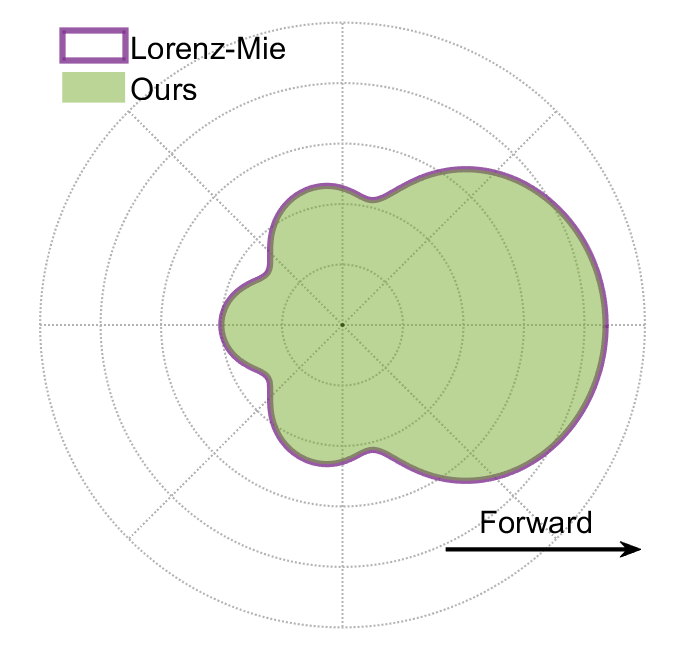
\includegraphics[width=\resLen]{pfunc/mie_300nm.png} & 
        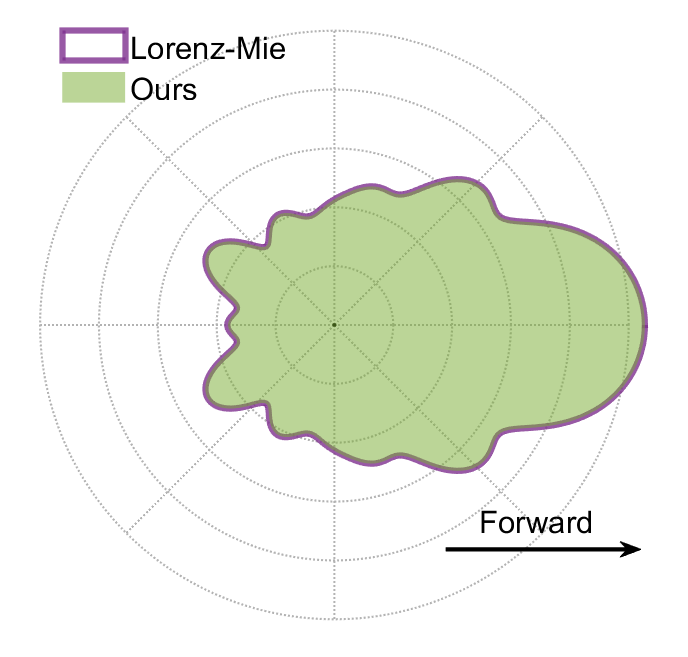
\includegraphics[width=\resLen]{pfunc/mie_600nm.png} &  
        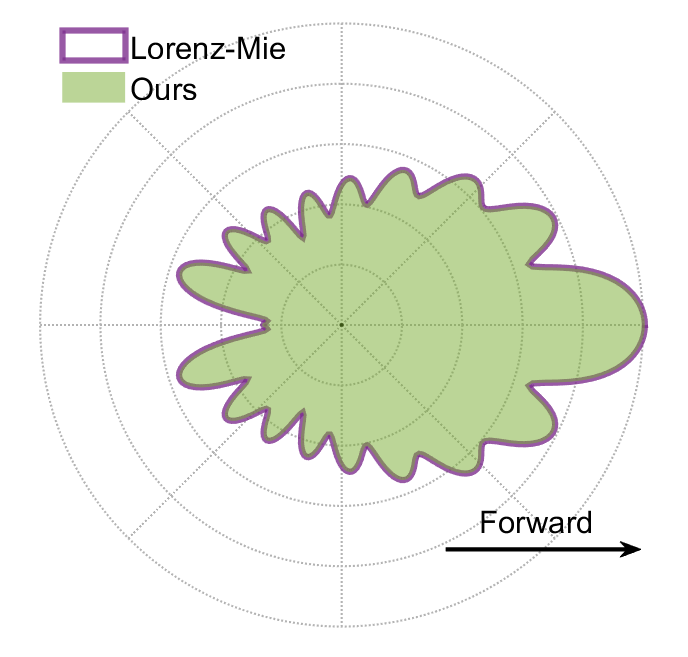
\includegraphics[width=\resLen]{pfunc/mie_900nm.png}  
        \\
        300nm & 600nm & 900nm
    \end{tabular}
    \caption{\label{fig:mie}
    Comparison against Lorenz-Mie theory: We compare our method with clusters containing a single particle (i.e., $\Ncls=1$) against a reference solution based on Lorenz-Mie theory for three different particle radii~$\radius_i \in \{ \text{300nm, 600nm, 900nm} \}$. As expected, for a single particle our method reduces to the same results as Lorenz-Mie theory. The wavelength is $\lambda=600$nm, while the refractive index of the particle is $\sIOR=1.5+0.1\img$.  
}
\end{figure}


\subsection{Relationship with the Radiative Transfer Theory}
\label{ssec:ours_RTT}
%
The scattering dyad $\ScaDyad_\Cls(\dwi,\dws)$ given by \Eq{eq:farscatdyadC} models how a particle cluster $\Cls$ scatters a planar unit-amplitude incident field in the far field region. However, for rendering we are generally interested on the average field intensity (i.e. radiance). 

As shown by Mishchenko~\shortcite{mishchenko2002vector}, the radiative transfer equation (RTE) directly derives from the far-field Foldy-Lax equations under three additional assumptions: (i)~The amount of coherent backscattering is negligible; (ii)~The particles are randomly distributed according to some distribution $p(\tPx_i,\Pprops_i)$, with $\tPx_i$ and $\Pprops_i$ denoting, respectively, the position and properties of a particle $i$; and (iii) We are interested on the average field $\EV{\EField(\px)}$. 

Following these assumptions, and after a lengthy derivation, Mishchenko demonstrates that the bulk scattering properties can be obtained from the far-field Foldy-Lax form, and in particular from the scattering dyad $\ScaDyad(\dwi,\dws)$. Let us first assume that the distribution of particle properties $\Pprops_i$ are independent of the particles position, and compute the average scattering dyad $\EV{\ScaDyad(\dwi,\dws)} = \int_\Omega \ScaDyad_i(\dwi,\dws) p(\Pprops_i) \diff{\Pprops_i}$. 
%
Then, note that the Foldy-Lax equation for clusters of particles~\eqref{eq:foldylaxcluster}, we derived above has the same form as the original Foldy-Lax equation~\eqref{eq:foldylax}. Thus, by the same derivation followed by Mishchenko we get to an equivalent RTE based on the scattering dyad of clusters. 

\paragraph{Computing the scattering parameters}
By taking the vectors of the parallel and perpendicular polarization $\dir{\boldsymbol\theta}^\text{inc}$ and $\dir{\boldsymbol\phi}^\text{inc}$ of the incident field as shown in Figure~\ref{fig:diagram} (right), and equivalently for the scattered field $\dir{\boldsymbol\theta}^\text{sca}$ and $\dir{\boldsymbol\phi}^\text{sca}$, we can compute the polarized scattering components $\ScaMatrix_\theta$ and $\ScaMatrix_\phi$ from the cluster's scattering dyad $\ScaDyad_\Cls(\dwi,\dws)$ as
%
\begin{align}
  \ScaMatrix_\theta(\dwi,\dws) &= \dir{\boldsymbol\theta}^\text{sca} \cdot \EV{\ScaDyad_\Cls(\dwi,\dws)} \cdot \dir{\boldsymbol\theta}^\text{inc}, \nonumber \\
  \ScaMatrix_\phi(\dwi,\dws) &= \dir{\boldsymbol\phi}^\text{sca} \cdot \EV{\ScaDyad_\Cls(\dwi,\dws)} \cdot \dir{\boldsymbol\phi}^\text{inc}.
\end{align}
%
Then, based on the two scattering components $\ScaMatrix_\theta$ and $\ScaMatrix_\phi$, we can obtain the optical parameters of the medium as
%
\begin{align}
    \label{eq:crosstcluster}
    \cT(\dwi) &= 4\pi \Re\left[\frac{\ScaMatrix(\dwi,\dwi)}{k_i^2}\right], \\
    \label{eq:crossscluster}
    \cS(\dwi) &=\int_\Sph \frac{|\ScaMatrix_\theta(\dwi,\dws)|^2+|\ScaMatrix_\phi(\dwi,\dws)|^2}{2k_1^2} \diff{\dws}, \\
    \label{eq:phasecluster}
    \phase(\dwi,\dws) &= \frac{|\ScaMatrix_\theta(\dwi,\dws)|^2+|\ScaMatrix_\phi(\dwi,\dws)|^2}{2k_1^2\cS},
\end{align}
%
with $\ScaMatrix(\dwi,\dwi)=\ScaMatrix_\phi(\dwi,\dwi)=\ScaMatrix_\theta(\dwi,\dwi)$, and $\Re[x]$ returning the real part of a complex number $x$. Lastly, assuming a uniform distribution of clusters, we can compute the extinction and scattering coefficients as
%
\begin{align}
    \label{eq:sigmatcluster}
    \sigT(\dwi) &= \cT(\dwi) \frac{\rho}{\EV{\Ncls}}, \\
    \label{eq:sigmascluster}
    \sigS(\dwi) &= \cS(\dwi) \frac{\rho}{\EV{\Ncls}},
\end{align}
%
with $\rho$ the number of particles per differential volume, and $\EV{\Ncls}$ the average number of particles per cluster. Note that the optical properties defined in Equations~\eqref{eq:crosstcluster}--\eqref{eq:sigmascluster} are directionally dependent, so they are general and can represent both isotropic and anisotropic media. 

\begin{figure}
    \centering
    \setlength{\resLen}{3.5in}
    \addtolength{\tabcolsep}{-3pt}
    \begin{tabular}{c}
        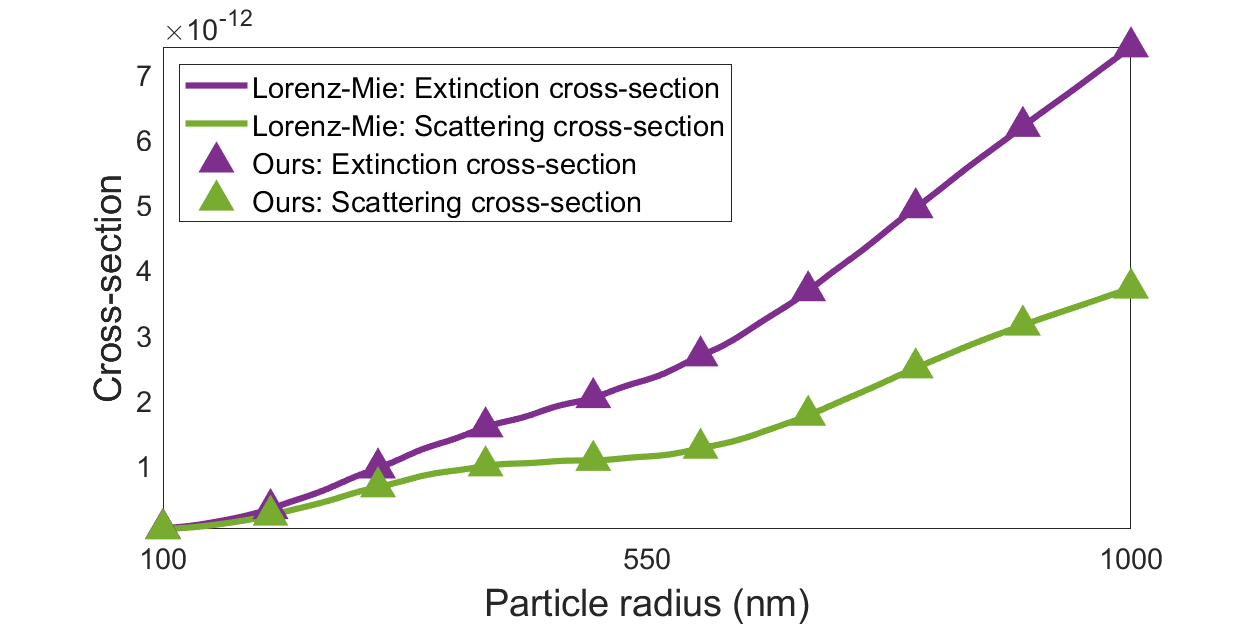
\includegraphics[width=\resLen]{pfunc/CsCt.png} 
    \end{tabular}
    \caption{
        Comparison against Lorenz-Mie theory: We compare the extinction and scattering cross sections computed with our method for $\Ncls=1$ against the results obtained using Lorenz-Mie theory. As in Figure~\ref{fig:mie} our results show perfect agreement. 
    \label{fig:mie2}
}
\end{figure}

\begin{figure*}[t]
    \centering
    \setlength{\resLenTwo}{2in}
    \setlength{\resLen}{.1\textwidth}
    \addtolength{\tabcolsep}{-3pt}
    \small
    \begin{tabular}{ccc|ccc|ccc}
        \multicolumn{3}{c|}{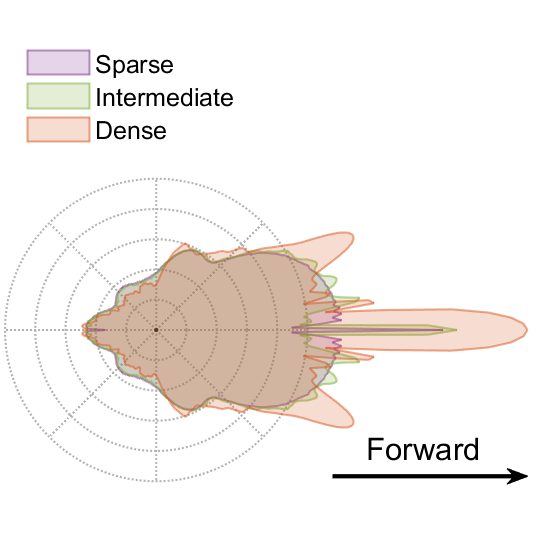
\includegraphics[width=3.\resLen]{pfunc/distance.png}} &
        \multicolumn{3}{c|}{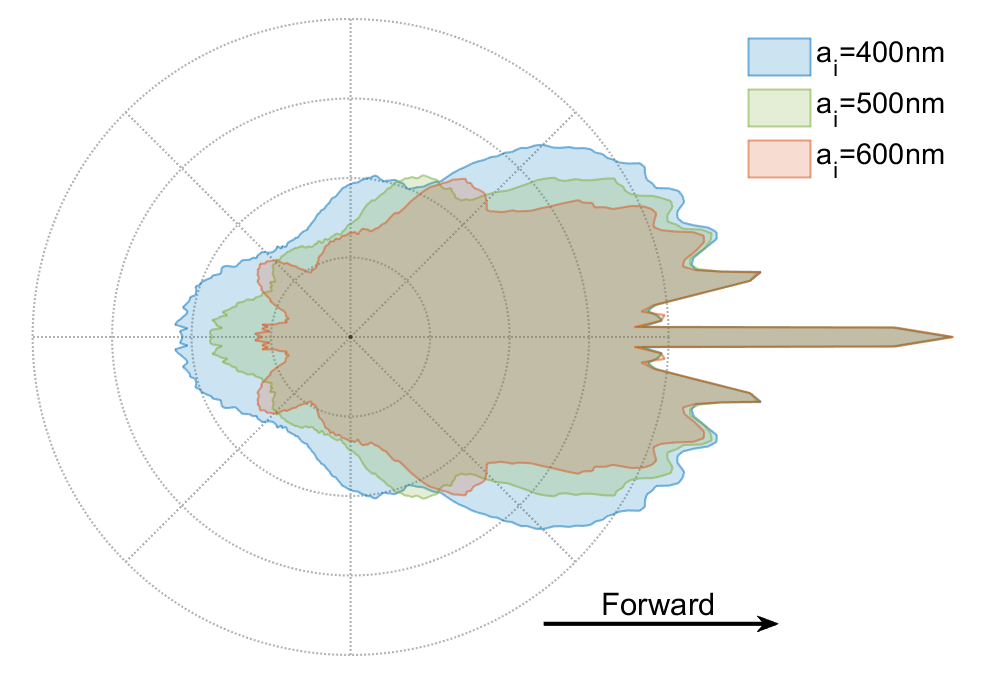
\includegraphics[width=3.\resLen]{pfunc/radius.png}} &
        \multicolumn{3}{c}{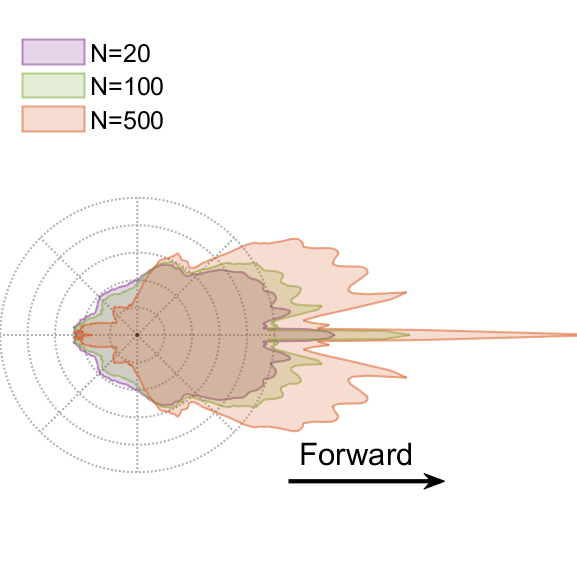
\includegraphics[width=3.\resLen]{pfunc/number.png}} \\[-5pt]
        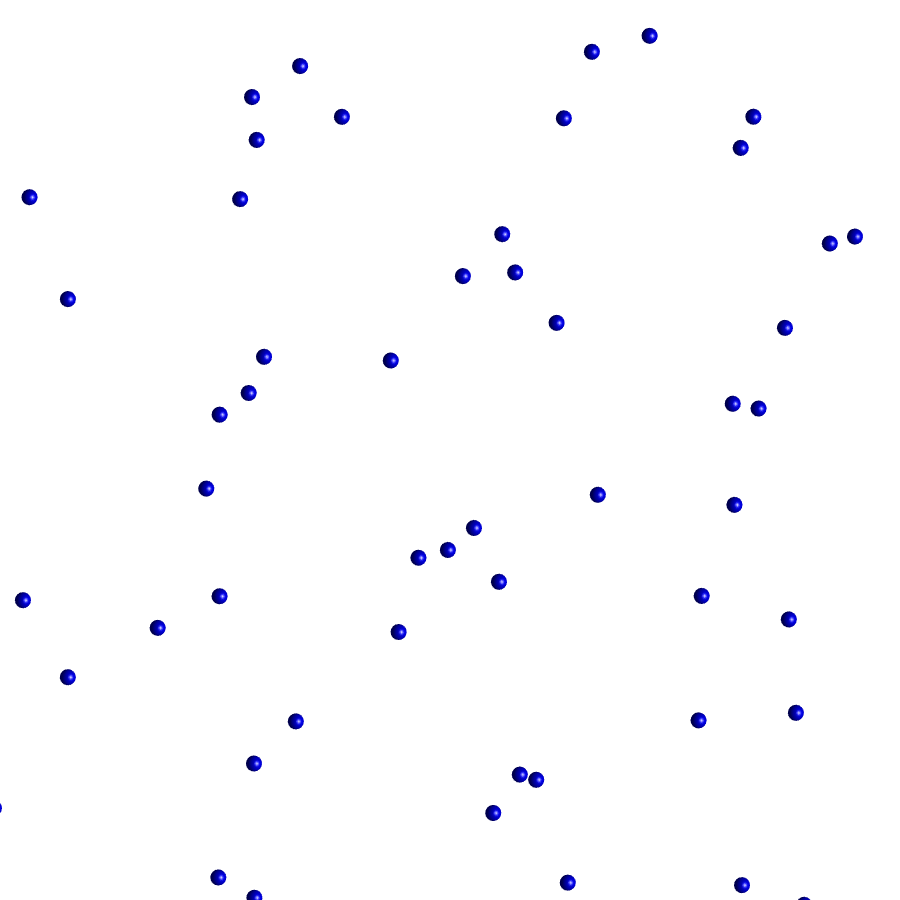
\includegraphics[width=\resLen]{particle/validate2_D1_N100_500nm.png} &
        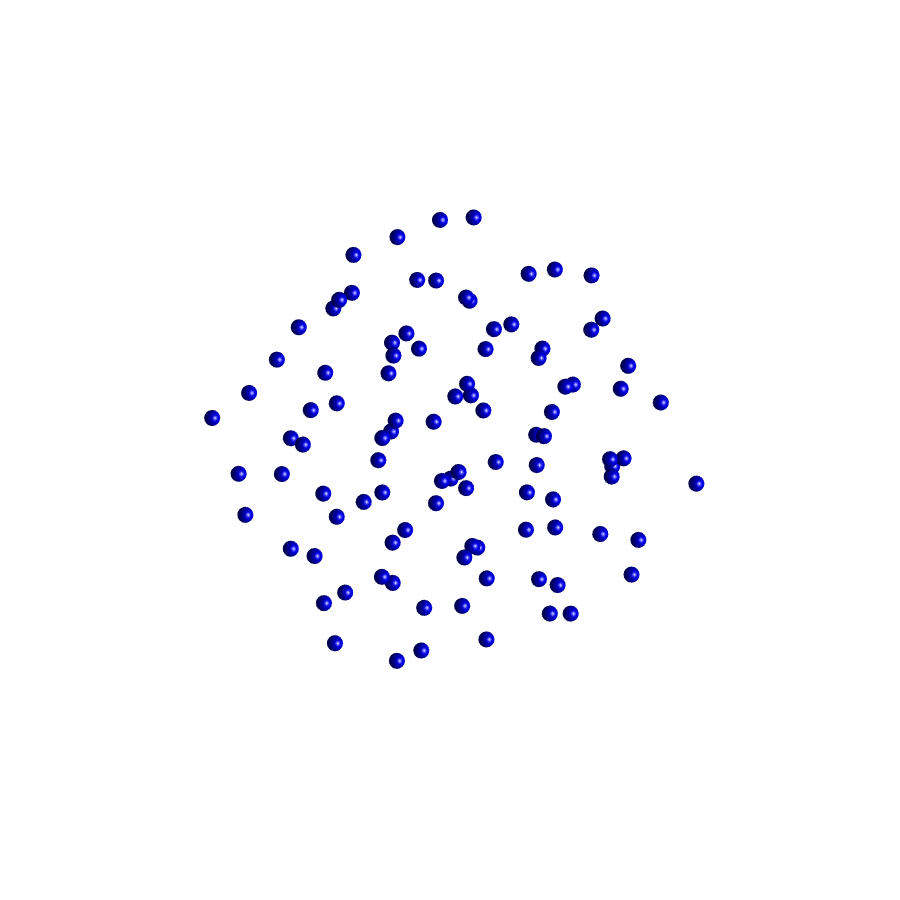
\includegraphics[width=\resLen]{particle/validate3_D2_N100_500nm.png} &
        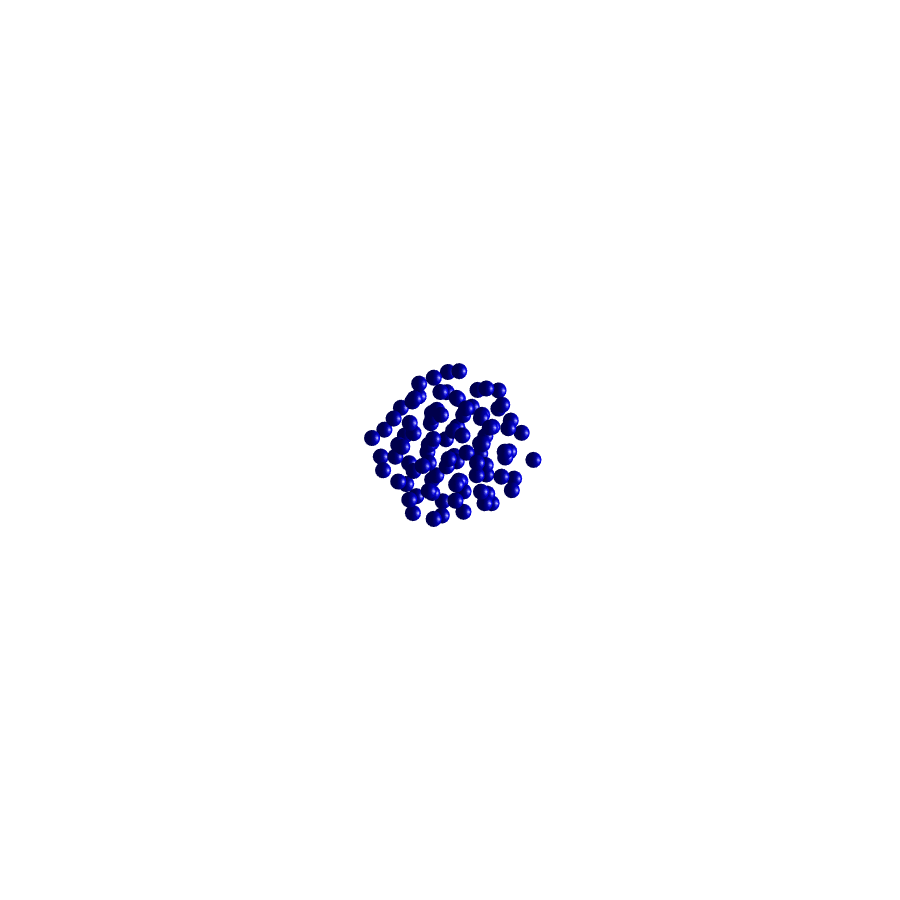
\includegraphics[width=\resLen]{particle/validate4_D3_N100_500nm.png} &
        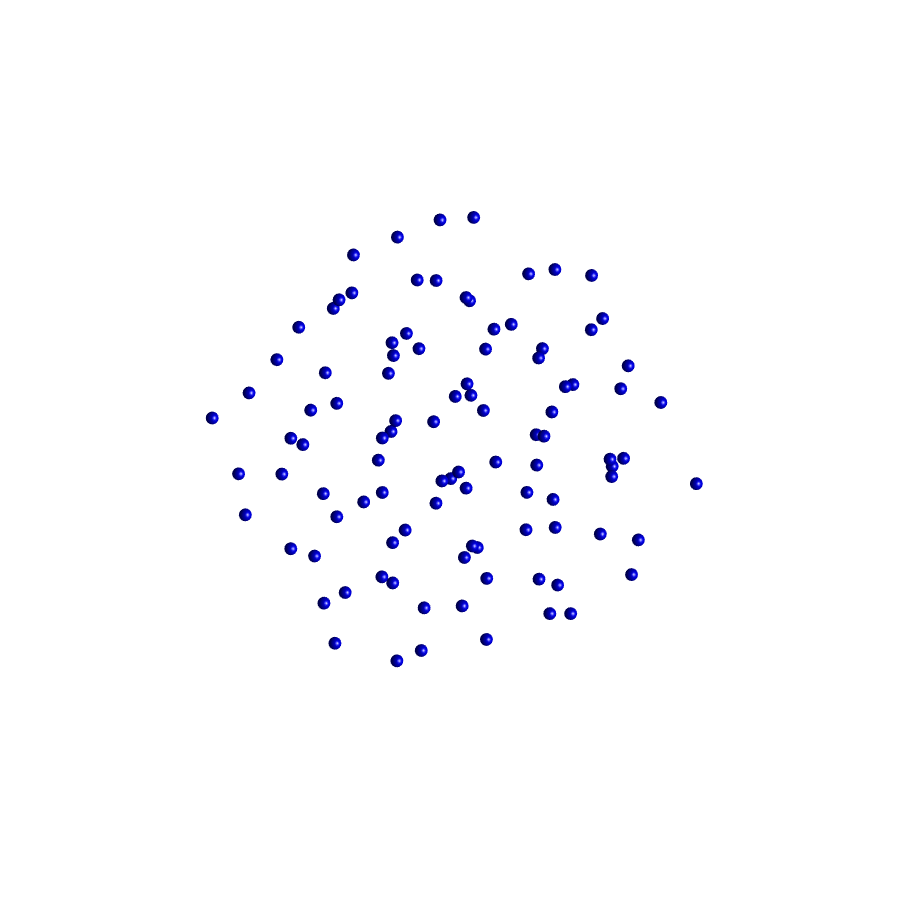
\includegraphics[width=\resLen]{particle/validate5_D2_N100_400nm.png} &
        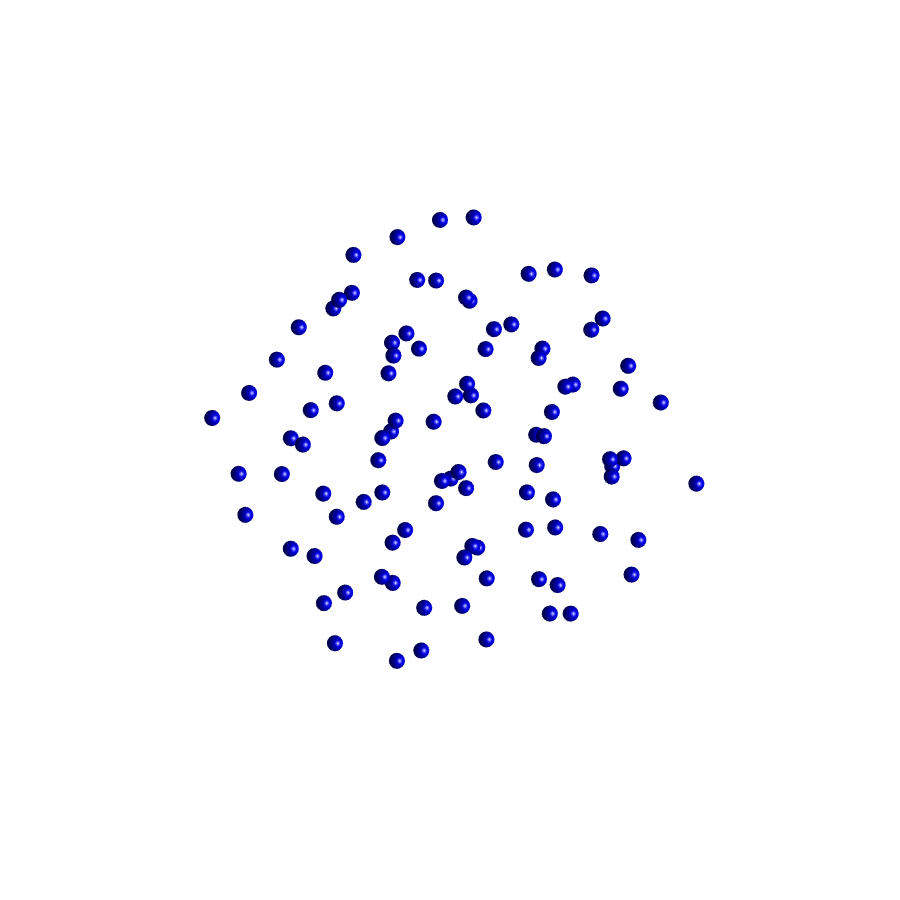
\includegraphics[width=\resLen]{particle/validate3_D2_N100_500nm.png} &
        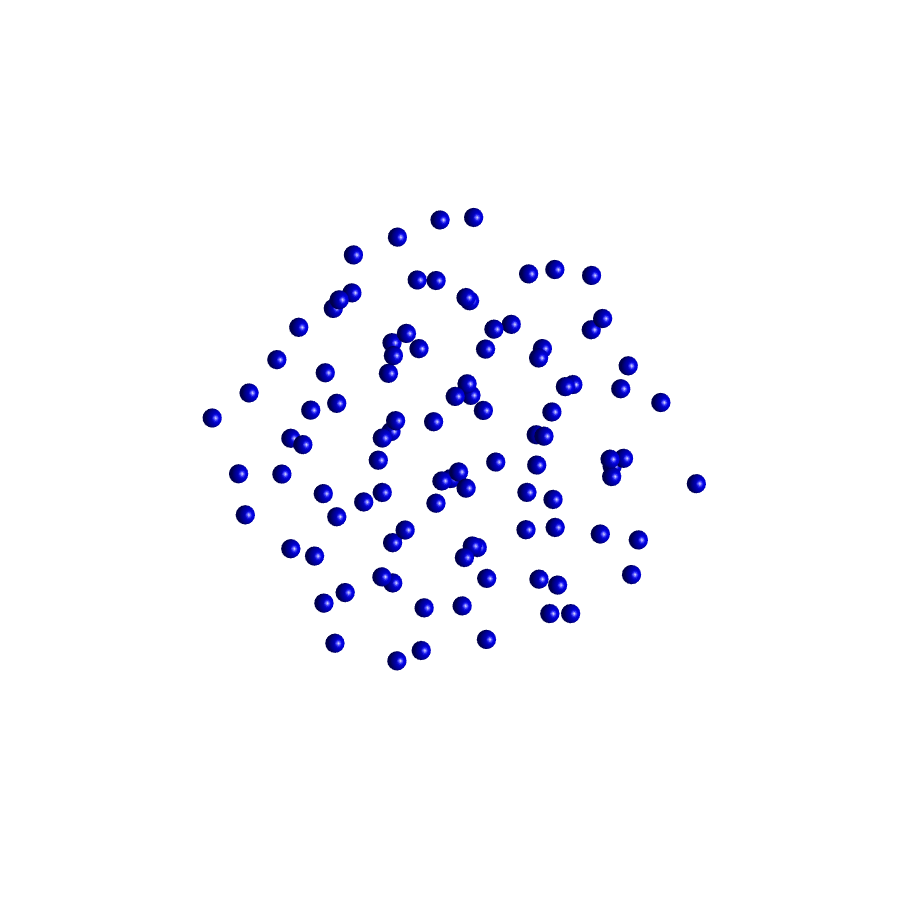
\includegraphics[width=\resLen]{particle/validate7_D2_N100_600nm.png} &
        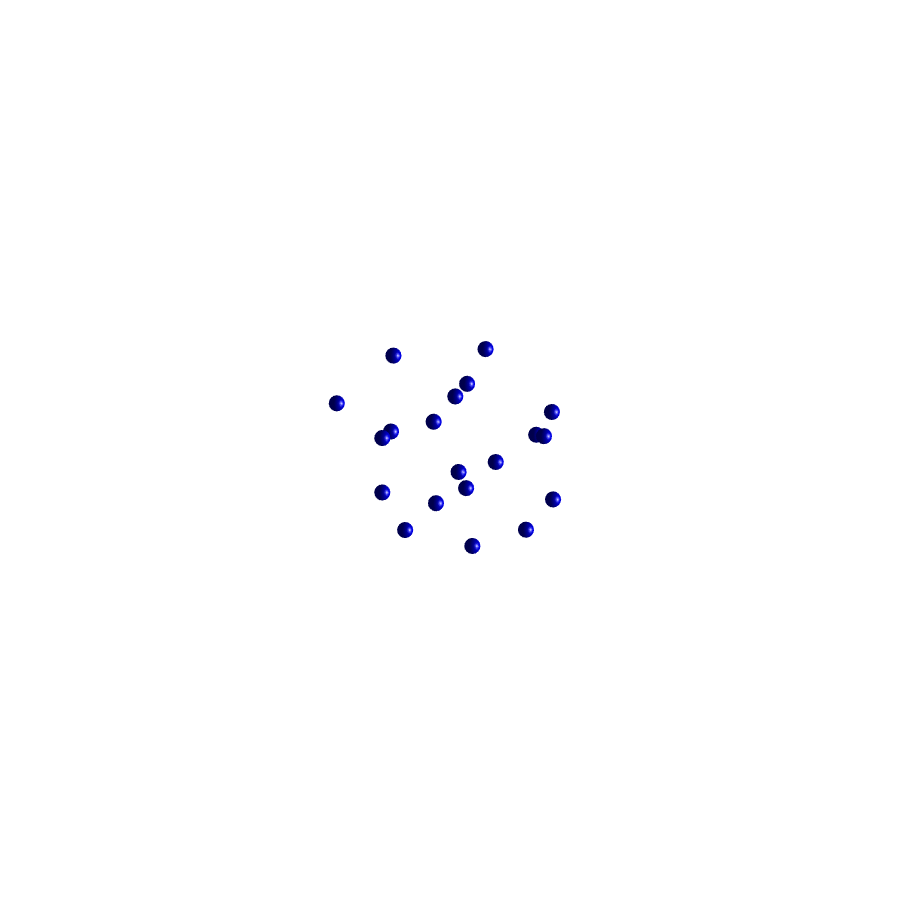
\includegraphics[width=\resLen]{particle/validate8_D2_N20_500nm.png} &
        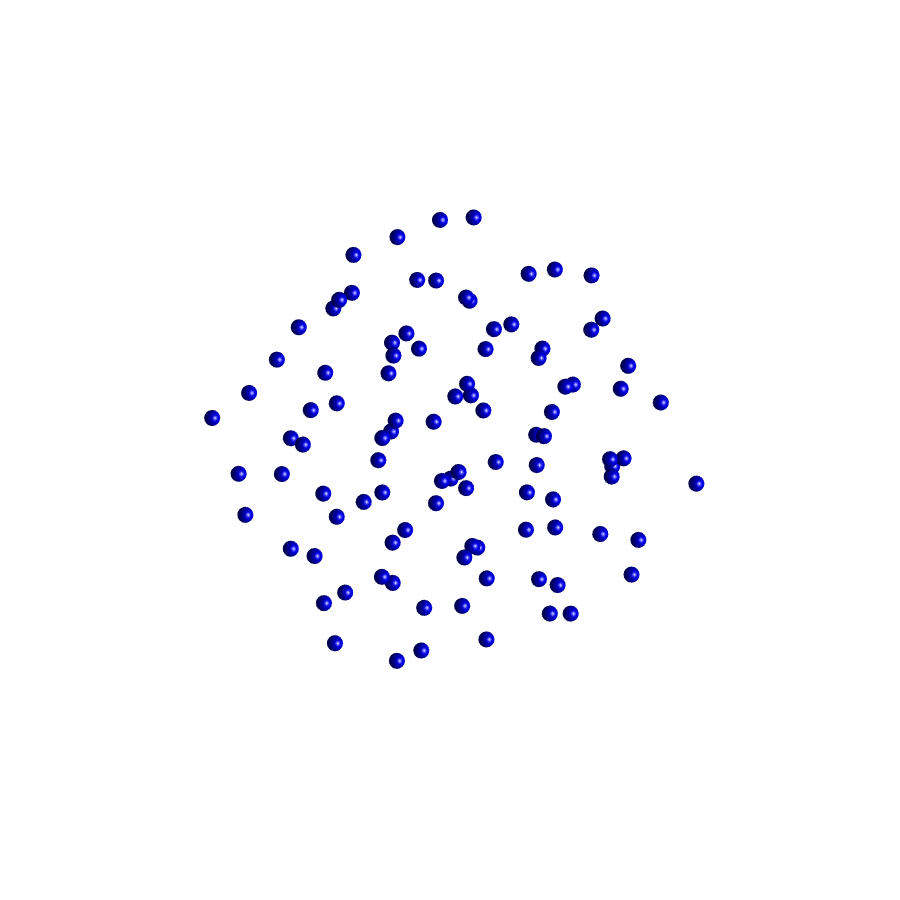
\includegraphics[width=\resLen]{particle/validate3_D2_N100_500nm.png} &
        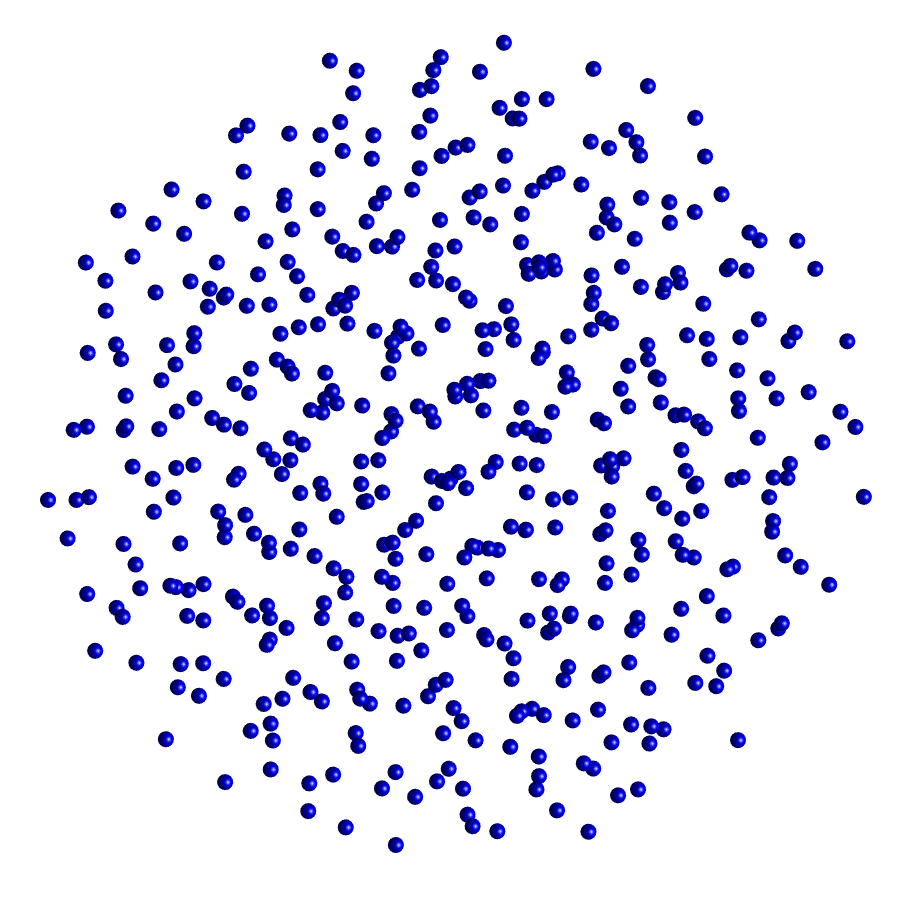
\includegraphics[width=\resLen]{particle/validate10_D2_N500_500nm.png} 
        \\
        Sparse & Intermediate & Dense & $\radius_i$=400nm & $\radius_i$=500nm & $\radius_i$=600nm &
        $\Ncls=20$ & $\Ncls=100$ & $\Ncls=500$ \\[5pt]
        \multicolumn{3}{c}{\bfseries (a) Varying particle spacing} &
        \multicolumn{3}{c}{\bfseries (b) Varying particle radii} &
        \multicolumn{3}{c}{\bfseries (c) Varying particle counts}
    \end{tabular}
    \caption{\label{fig:ablation}
        Comparison of the resulting \rev{(normalized)} phase function for different cluster parameters, for a planar incident field at $\lambda=700$nm. Unless mentioned otherwise, the clusters have $\Ncls=100$ particles, and each particle has radius $\radius_i=500$nm. For each phase function, we vary: (a) The distance between particles within the cluster; (b) The particle size $\radius_i$; and (c) The number of particles $\Ncls$.
        \rev{We visualize all phase functions in logarithmic scale to better show their low-magnitude regions.}
    }
\end{figure*}

\subsection{Relationship with Independent Scattering}
\label{ssec:ours_indep_scat}
%
Most previous works rendering light transport in media~\cite{novak2018monte} build on the assumption of independent scattering---that is, particles are in their respective far-field region.
It is easy to verify that this is a special case of \Eq{eq:foldylaxtwo} with $\Ncls=1$, causing 
the scattering dyad $\ScaDyad_\Cls$ of \Eq{eq:farscatdyadC} to reduce to
%
\begin{equation}
    \label{eq:farscatmie}
    \ScaDyad_\Cls(\dwi,\dws) = \ScaDyad_i(\dwi,\dws) = \frac{g(\dws)\cdot \dyad{T}_i  \cdot\sGreenProp(\dwi)}{4\pi},
\end{equation}
%
which encodes the scattered field in the far-field region of a particle when excited by an incident unit-amplitude planar field. 
%
The Lorenz-Mie theory~\cite{hulst1981light} provides closed-form expressions for $\ScaDyad_i(\dwi,\dws)$ for spheres and cylinders, while numerical solutions of $\ScaDyad_i(\dwi,\dws)$ have been proposed for scatterers of arbitrary shapes via, for example, the T-matrix method~\cite{waterman1965matrix}, or more recently based on the BEM for cylindrical fibers~\cite{xia2020wave}. Our work is therefore a generalization of these works to particles in the near field. 

    \section{Computing the Bulk Scattering Parameters}
\label{sec:ours_numerical}
%
We now detail our numerical computations of the scattering dyad $\ScaDyad_\Cls(\dwi,\dws)$ of \Eq{eq:farscatdyadC}, \rev{which in turn determines the bulk scattering parameters following Equations~\eqref{eq:crosstcluster}--\eqref{eq:sigmascluster}. These bulk scattering parameters}can be directly used in any renderer supporting participating media~\cite{novak2018monte} \rev{using tabulated phase function and cross sections.}

Computing $\ScaDyad_\Cls(\dwi,\dws)$ essentially boils down to solving the time-harmonic Maxwell equations for an incident unit-amplitude planar field with direction $\dwi$. While several different methods exist for that purpose (see \S 16 of~\cite{mishchenko2014electromagnetic} for an overview), we opt for the superposition T-matrix method~\cite{mackowski1996calculation} that has been demonstrated efficient for moderately large $\Ncls$, can handle scatterers with arbitrary geometry, and is based on the principles of the Foldy-Lax equations, making it particularly appealing for our work. 

In practice, we use the open-source CUDA-based \texttt{CELES} solver \cite{egel2017celes}, which implements the superposition T-matrix method proposed by Mackowski and Mishchenko \shortcite{mackowski2011multiple} for spherical or randomly rotated particles.
In our implementation, we focus on clusters of spherical particles.
Since the Lorenz-Mie theory also assumes spherical particles, this allows us to directly compare our results with those computed using the Lorenz-Mie theory \rev{(see Figures~\ref{fig:mie} and \ref{fig:mie2}). Note that the T-matrix method does not introduce assumptions on the size of particles but, similar to Lorenz-Mie theory, larger particles result in more expensive computations. }

To compute the average scattering dyad $\EV{\ScaDyad_\Cls(\dwi,\dws)}$, we average the scattered field of several random realizations of the clusters (each of which obtained by randomly sampling the position of the particles inside the cluster's bounding sphere).
As we will demonstrate in \S\ref{sec:result}, we use a wide array of distributions including particles uniformly distributed over the volume of the cluster, positively-correlated particles following Shaw et al.~\shortcite{shaw2002super}, negatively-correlated particles using Poisson sampling of the sphere, and anisotropic distributions by uniformly sampling the particles on a oriented 2D disk.

Lastly, we represent the resulting phase function as well as the extinction and scattering cross sections as tabulated (i.e., piecewise constant) functions that can be used for rendering.

%\AJ{Maybe add some detail on the tabulation? How many angular bins do we use? How much in the case of anisotropic PFs?How much on the spectral domain?} \sz{Yes, we should provide some details here.}

    \section{Experiments}
\label{sec:result}
%
In this section, we first validate our technique by comparing bulk scattering parameters computed with our method and the Lorenz-Mie theory (\S\ref{ssec:result_validation}).
Then, we apply our technique described in \S\ref{sec:ours_theory} and \S\ref{sec:ours_numerical} to compute bulk scattering parameters for a wide range of participating media (\S\ref{ssec:result_main}).

\begin{figure}
    \centering
    \setlength{\resLen}{1.55in}
    \setlength{\raiseLen}{.75in}
    \addtolength{\tabcolsep}{-3.5pt}
    \small
	\begin{tabular}{ccccc}
		& $\Ncls=1$ & $\Ncls=50$ & $\Ncls=100$ & $\Ncls=500$
		\\
		\raisebox{\raiseLen}{\rotatebox[origin=c]{90}{$\radius_i=300\text{nm}$}} &
		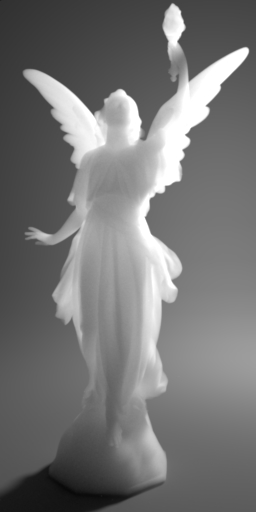
\includegraphics[height=\resLen]{lucy/N1_300nm.jpg} &
		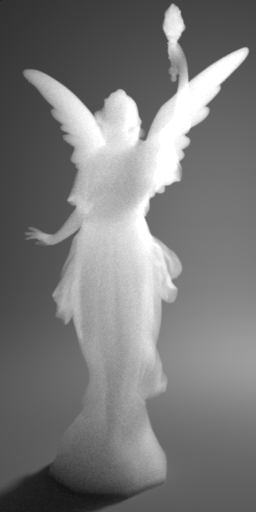
\includegraphics[height=\resLen]{lucy/N50_300nm.jpg} &
		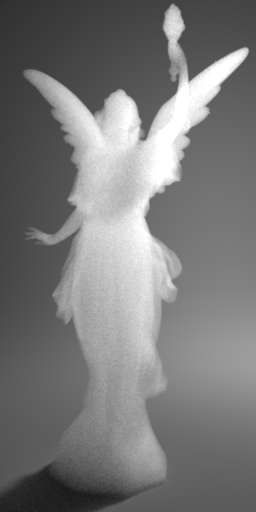
\includegraphics[height=\resLen]{lucy/N100_300nm.jpg} &
		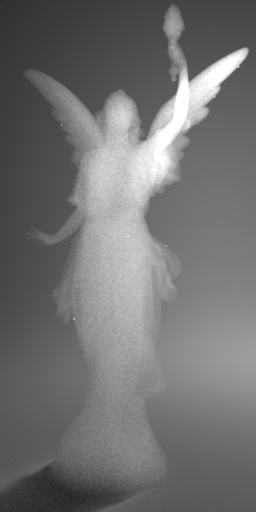
\includegraphics[height=\resLen]{lucy/N500_300nm.jpg}
		\\
		\raisebox{\raiseLen}{\rotatebox[origin=c]{90}{$\radius_i=400\text{nm}$}} &
		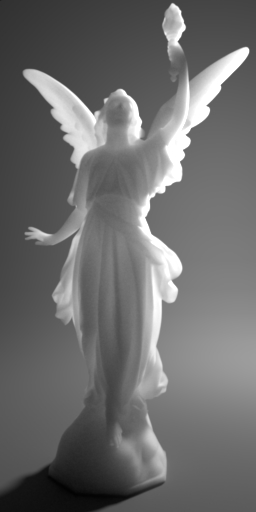
\includegraphics[height=\resLen]{lucy/N1_400nm.jpg} &
		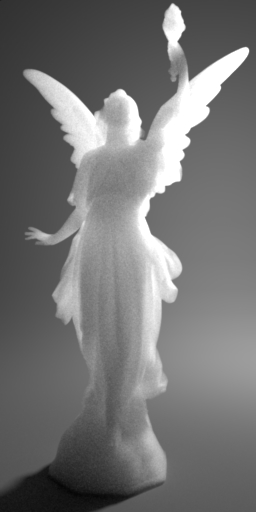
\includegraphics[height=\resLen]{lucy/N50_400nm.jpg} &
		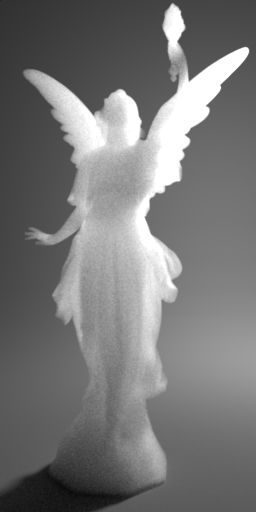
\includegraphics[height=\resLen]{lucy/N100_400nm.jpg} &
		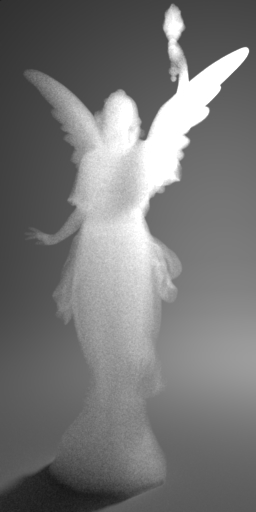
\includegraphics[height=\resLen]{lucy/N500_400nm.jpg}
		\\
		\raisebox{\raiseLen}{\rotatebox[origin=c]{90}{$\radius_i=500\text{nm}$}} &
		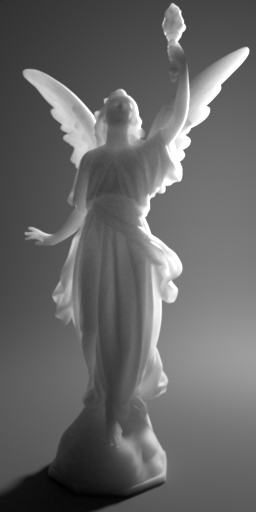
\includegraphics[height=\resLen]{lucy/N1_500nm.jpg} &
		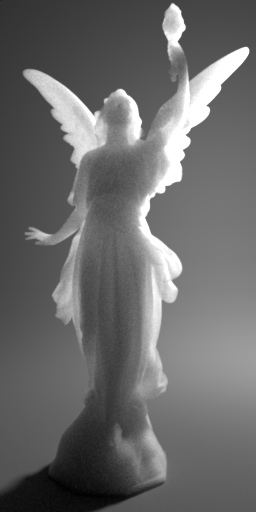
\includegraphics[height=\resLen]{lucy/N50_500nm.jpg} &
		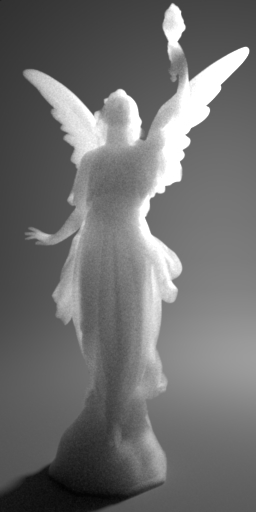
\includegraphics[height=\resLen]{lucy/N100_500nm.jpg} &
		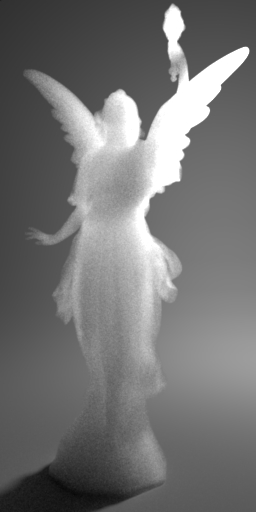
\includegraphics[height=\resLen]{lucy/N500_500nm.jpg}
	\end{tabular}
    \caption{\label{fig:lucycompare}
        Renderings of homogeneous Lucy models at $\lambda = 700\text{nm}$.
        The bulk scattering parameters are computed using our method with different combinations of particle radius~$\radius_i$ and per-cluster particle count~$\Ncls$.
    }
\end{figure}


\subsection{Validation}
\label{ssec:result_validation}
%
To validate our technique, we compare computed bulk scattering parameters provided by our implementation and \texttt{MiePlot}~\cite{laven2011mieplot}, a free software based on the Lorenz-Mie theory.
We focus on the configuration where a cluster contains only one (spherical) particle as this is a fundamental assumption of the Lorenz-Mie theory.

In Figure~\ref{fig:mie}, we visualize computed single-scattering phase functions at the wavelength 600~nm with three particle radii (300, 600, and 900~nm).
We set the refractive index of the embedding medium to $(1.5 + 0.1\img)$.
Additionally, we show in Figure~\ref{fig:mie2} the corresponding extinction and scattering cross sections $\cT$ and $\cS$ given by Equations~\eqref{eq:crosstcluster} and \eqref{eq:crossscluster}, respectively.
In all these examples, our computed scattering parameters match those predicted by the Lorenz-Mie theory perfectly.

\subsection{Main Results}
\label{ssec:result_main}
%
We now demonstrate the versatility of our technique by computing bulk scattering parameters for a range of participating media.
Please see Table~\ref{fig:time} for the performance statistics of our experiments.

\begin{figure}
    \centering
    \setlength{\resLen}{1.2in}
    \addtolength{\tabcolsep}{-3pt}
    \small
    \begin{tabular}{cc}
        \begin{overpic}[height=\resLen]{pfunc/color.png}
            \put(2, 57){Ours}
        \end{overpic}
        &
        %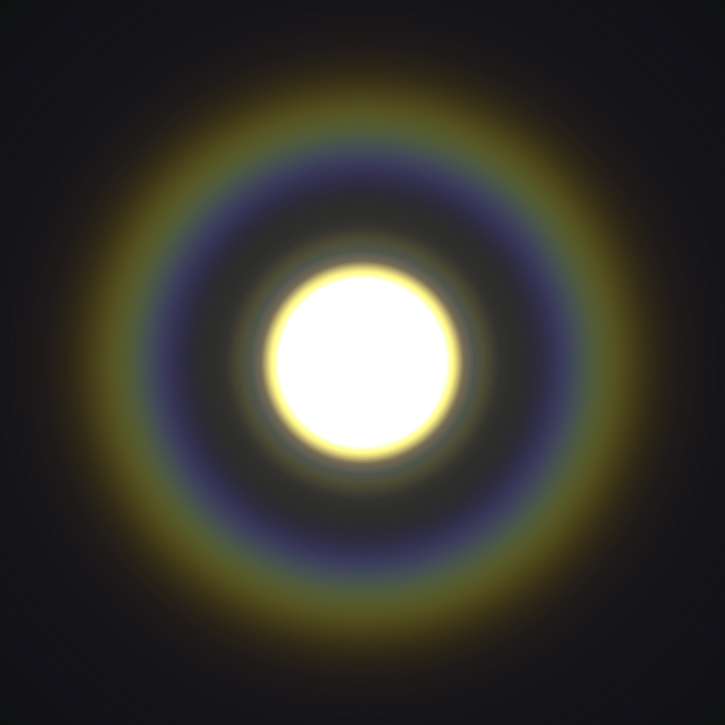
\includegraphics[height=\resLen]{slab/color.jpg} &
        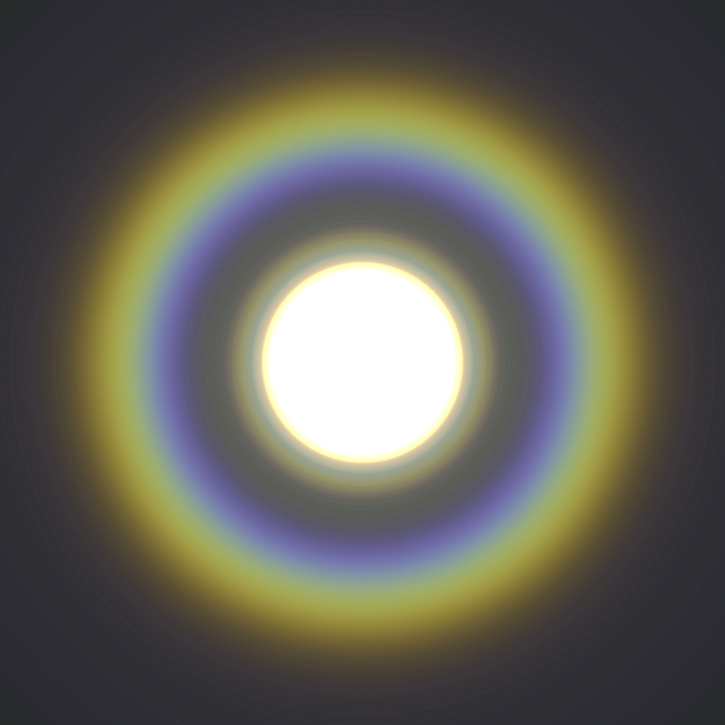
\includegraphics[height=\resLen]{slab/color4x.jpg}
        \\
        \begin{overpic}[height=\resLen]{pfunc/color1.png}
            \put(2, 57){Single-particle}
        \end{overpic}
        &
        %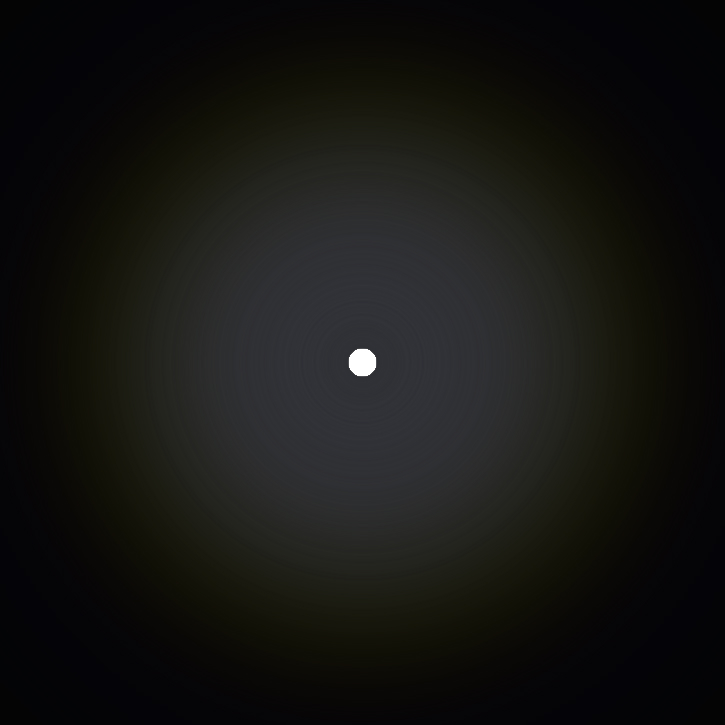
\includegraphics[height=\resLen]{slab/color_1.jpg} &
        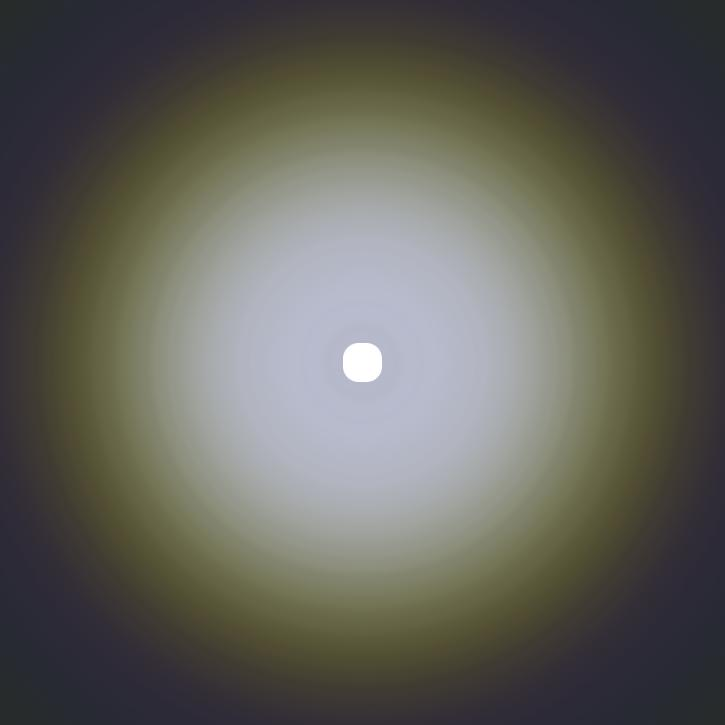
\includegraphics[height=\resLen]{slab/color4x_1.jpg}
        \\
        \textbf{(a) Phase function} & \textbf{(b) Thin-slab rendering}
    \end{tabular}
    \caption{\label{fig:multiwave1}
        \textbf{Multi-spectral results:} (a) visualizations of phase functions; (b) corresponding multi-spectral renderings of a thin slab lit by a small area light from behind.
        Results on the top are generated using a cluster of 100 particles with radii 500nm.
        Results on the bottom are obtained using a conventional single-particle setting.
        We used identical particle counts per differential volume for both configurations.
    }
\end{figure}

\begin{figure}
    \centering
    \setlength{\resLen}{0.8in}
    \setlength{\raiseLen}{0.9in}
    \addtolength{\tabcolsep}{-3.5pt}
    \small
    %
    \begin{tabular}{cccc}
        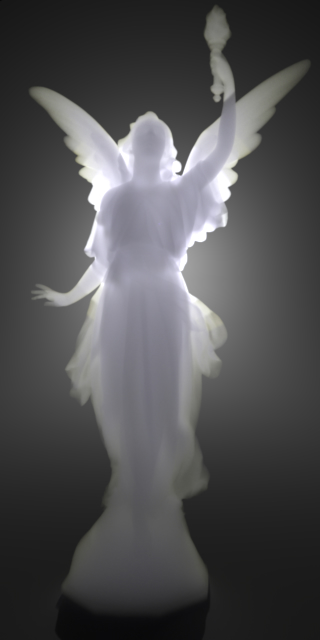
\includegraphics[width=\resLen]{lucy/color.jpg} &
        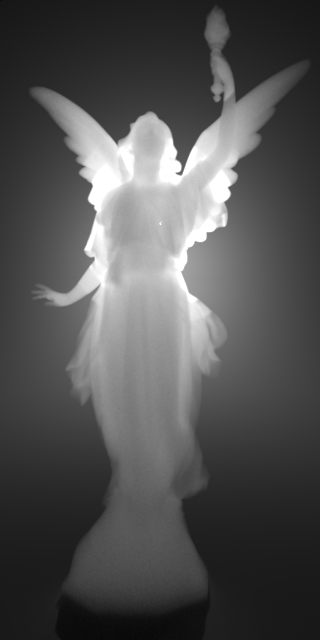
\includegraphics[width=\resLen]{lucy/color_400nm.jpg} &
        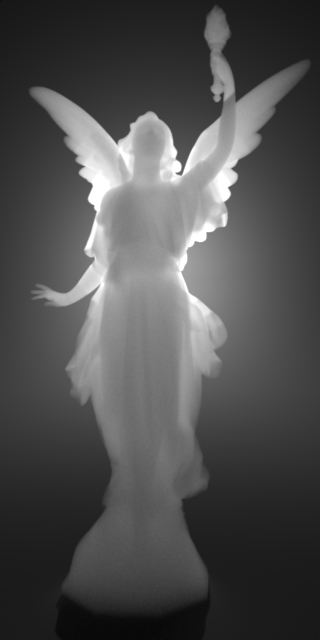
\includegraphics[width=\resLen]{lucy/color_550nm.jpg} &
        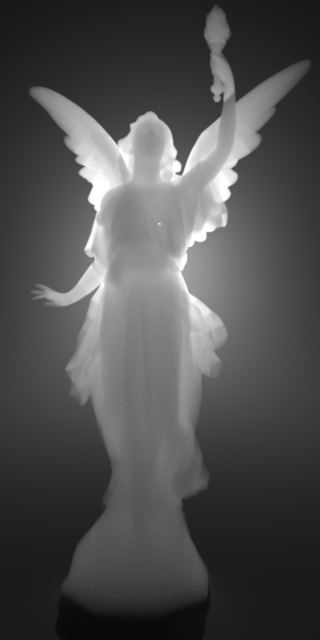
\includegraphics[width=\resLen]{lucy/color_700nm.jpg}
        \\
        \textbf{(a) Multi.} & \textbf{(b) 400nm} & \textbf{(c) 550nm} & \textbf{(d) 700nm}
    \end{tabular}
    \caption{\label{fig:multiwave2}
        (a)~Multi-spectral rendering of a homogeneous Lucy model using identical bulk scattering parameters as the top row of Figure~\ref{fig:multiwave1}.
        (b--d)~Monochrome renderings of the same model at three wavelengths.
    }
\end{figure}

% \raisebox{\raiseLen}{\multirow{2}{*}{\includegraphics[width=\resLen]{lucy/color.jpg}}} & \includegraphics[width=\resLen]{placeholder3.jpg} \\
% & \includegraphics[width=\resLen]{placeholder3.jpg}


\paragraph{Isotropic media}
In computer graphics, volumetric light transport effects are typically simulated using \emph{isotropic media} where the extinction and scattering coefficients $\sigT$, $\sigS$ are directionally independent, and the single-scattering phase function $\phase$ is formulated as a 1D function on the angle between the incident and scattered directions.

Our technique can produce bulk scattering parameters for isotropic media using particles distributed in radically symmetric densities.
We conduct a few ablation studies to demonstrate how different particle arrangements in a cluster affects the resulting parameters.
We use a wavelength of 600~nm for all these studies and represent the 1D phase functions as tabulated (i.e., piecewise constant) functions using 180 equal-sized bins.

In our first study, we use a cluster of 100 particles with radii 500~nm. Then, we vary the distances between particles (by using bounding spheres with different sizes and distributing particles uniformly in these spheres).
As shown in Figure~\ref{fig:ablation} (a), the closer the particles are to each other, the more forward the resulting phase function is.
This is expected: With sparsely distributed particles, it is simpler for light to pass straightly through.

Our second ablation study examines the effect of particle size. With 100 uniformly distributed particles, we apply our technique to three particle sizes ($\radius_i$= 400, 500, and 600 nm).
As shown in Figure~\ref{fig:ablation} (b), as we increase the particles radius, the phase function becomes more forward and increases its frequency. This agrees with the behaviour of single particles predicted by Lorenz-Mie theory. 

In our third study, we vary the number of particles in a cluster while keeping the particle size fixed to $\radius_i$=500 nm.
Figure~\ref{fig:ablation} (c) shows that as we increase the number of particles, the phase function gets more forward and of higher-frequency, in a behaviour somewhat correlated with the particles size. This is the result of the increasing number of diffractive elements on the cluster, that instead of making scattering more diffuse (as predicted by geometric optics) increases its forward frequency. 

Lastly, we show in Figure~\ref{fig:lucycompare} monochrome renderings using bulk scattering parameters obtained with varying combinations of particle count and radius.

\begin{figure}[t]
    \centering
    \setlength{\resLen}{1in}
    \addtolength{\tabcolsep}{-3pt}
    \small
    \begin{tabular}{ccc}
        & Forward & Backward\\
        \includegraphics[height=.9\resLen]{particle/aniso_z.png}
        & \multicolumn{2}{c}{\includegraphics[height=\resLen]{pfunc/aniso_z.png}}
        %& \includegraphics[height=\resLen]{slab/aniso_z.jpg}
        \\
        \includegraphics[height=.9\resLen]{particle/aniso_y.png}
        & \multicolumn{2}{c}{\includegraphics[height=\resLen]{pfunc/aniso_y.png}}
        %& \includegraphics[height=\resLen]{slab/aniso_y.jpg}
        \\
        \textbf{(a) Incident direction} & \multicolumn{2}{c}{\textbf{(b) Phase function slice}}
    \end{tabular}
    \caption{\label{fig:aniso1}
        Visualizations of slices $\phase(\dwi,\cdot)$ of a phase function for two incident directions~$\dwi$ at $\lambda = 700\text{nm}$.
        This phase function is computed using a configuration where 100 particles with radii 500nm follow an anisotropic Gaussian distribution.
    }
\end{figure}

\begin{figure}[t]
    \centering
    \setlength{\resLen}{1.06in}
    \addtolength{\tabcolsep}{-3pt}
    \small
    \begin{tabular}{ccc}
        \begin{overpic}[width=\resLen]{lucy/aniso_x.jpg}
            \put(2,2){\color{white} \bfseries x}
        \end{overpic}
        &
        \begin{overpic}[width=\resLen]{lucy/aniso_y.jpg}
            \put(2,2){\color{white} \bfseries y}
        \end{overpic}
        &
        \begin{overpic}[width=\resLen]{lucy/aniso_z.jpg}
            \put(2,2){\color{white} \bfseries z}
        \end{overpic}
    \end{tabular}
    \caption{\label{fig:aniso2}
        Renderings of homogeneous Lucy models with the same anisotropic medium as in Figure~\ref{fig:aniso1}.
        With the medium's orientation---which determines the axis of the disk---aligned with the $x$-, $y$-, and $z$-axis, respectively, the Lucy model exhibit distinct appearances.
    }
\end{figure}


\paragraph{Multi-spectral results}
Since our technique is derived using microphysical wave optics, it allows systematic generation of multi-spectral parameters based on a single (monochrome) configuration of particle cluster.

To demonstrate this, we use a configuration of 100 uniformly distributed particles (per cluster) with radius 500~nm and compute bulk scattering parameters at 50 wavelengths ranging from 400~nm to 700~nm.
In Figure~\ref{fig:multiwave1}, we visualize the computed phase functions at three wavelengths as well as multi-spectral renderings of a backlit thin slab.
The smooth changes in scattering parameters across wavelength have resulted in a characteristic rainbow-like effect.
When using the single-particle configuration (with identical overall particle density per unit volume), the rainbow effect is missing.

Figure~\ref{fig:multiwave2} shows renderings of the Lucy model using these scattering parameters.

\paragraph{Anisotropic media}
Anisotropic media allow the extinction and scattering coefficients $\sigT$, $\sigS$ to be directionally dependent, and have full 4D phase functions~$\phase$.
Previously, although the scattering parameters of anisotropic media can be devised based on the microflake models~\cite{jakob2010radiative,heitz2015sggx}, equivalences of the Lorenz-Mie theory, to our knowledge, have been lacking. 

By using anisotropic particle distributions, our technique can generate bulk scattering parameters for anisotropic media.
To demonstrate this, we use a configuration where the cluster contains $\Ncls = 100$ particles following an anisotropic Gaussian distribution, as illustrated in Figure~\ref{fig:aniso1} (a).
We tabulate the extinction and scattering cross sections using the latitude-longitude parameterization with a resolution of $180 \times 360$.
Due to the symmetry of the disc, the resulting phase function~$\phase$ is three-dimensional, and we tabulated it with the resolution $90 \times 180 \times360$.

In Figure~\ref{fig:aniso1} (b), we visualize slices of the computed single-scattering phase function~$\phase$ with two incident directions~$\dwi$.
In Figure~\ref{fig:aniso2}, we show renderings of the Lucy model with three (spatially invariant) orientations.

\paragraph{Correlated particles}
Finally, in Figure~\ref{fig:correlated} we demonstrate the effect of particles correlation within the cluster, by analyzing particles distributed using both negative (Poisson sampled) and positive correlation~\cite{jarabo2018radiative}. We compare the effect of introducing microscopic correlation on media where the clusters position is itself correlated, compared with uniformly distributed particles inside the clusters. These two levels of correlation have significant effect on the final appearance of the translucent materials. 

%\sz{We need to report precomputation times.}
\begin{table}[t]
    \caption{\label{fig:time}
        Performance statistics for our simulation.
		The numbers are collected using a workstation equipped with an Intel i7-6800K six-core CPU and an Nvidia GTX 1080 GPU.
		To average the randomness of the particle position, we run 50 times for each simulation, so all the number should times 50 for the results in our paper.
    }
    \begin{tabular}{ccccc}
    \hline
                                                    & N     & $\phase$ res.    & time   \\
    Regular (Fig~\ref{fig:lucycompare})             & 1-500 &  180x360         & 3-16s  \\
    Multi-spectral (Fig~\ref{fig:multiwave1})       & 100   &  180x360x50      & 35mins \\
    Anisotropic (Fig~\ref{fig:aniso2})              & 100   &  180x360x90      & 13mins \\
    Correlated (Fig~\ref{fig:correlated})           & 100   &  180x360         & 98s    \\
    \hline
    \end{tabular}
\end{table}


%\begin{figure*}[t]
    \centering
    \setlength{\resLenTwo}{2in}
    \setlength{\resLen}{.1\textwidth}
    \addtolength{\tabcolsep}{-3pt}
    \small
    \begin{tabular}{ccc|ccc|ccc}
        \multicolumn{3}{c|}{\includegraphics[height=\resLenTwo]{images/pfunc/distance.png}} &
        \multicolumn{3}{c|}{\includegraphics[height=\resLenTwo]{images/pfunc/radius.png}} &
        \multicolumn{3}{c}{\includegraphics[height=\resLenTwo]{images/pfunc/number.png}} \\[-5pt]
        \includegraphics[width=\resLen]{images/particle/validate2_D1_N100_500nm.png} &
        \includegraphics[width=\resLen]{images/particle/validate3_D2_N100_500nm.png} &
        \includegraphics[width=\resLen]{images/particle/validate4_D3_N100_500nm.png} &
        \includegraphics[width=\resLen]{images/particle/validate5_D2_N100_400nm.png} &
        \includegraphics[width=\resLen]{images/particle/validate3_D2_N100_500nm.png} &
        \includegraphics[width=\resLen]{images/particle/validate7_D2_N100_600nm.png} &
        \includegraphics[width=\resLen]{images/particle/validate8_D2_N20_500nm.png} &
        \includegraphics[width=\resLen]{images/particle/validate3_D2_N100_500nm.png} &
        \includegraphics[width=\resLen]{images/particle/validate10_D2_N500_500nm.png} 
        \\
        Sparse & Intermediate & Dense & $\radius_i$=400nm & $\radius_i$=500nm & $\radius_i$=600nm &
        $\Ncls=20$ & $\Ncls=100$ & $\Ncls=500$ \\[5pt]
        \multicolumn{3}{c}{\bfseries (a) Varying particles spacing} &
        \multicolumn{3}{c}{\bfseries (b) Varying particles radius} &
        \multicolumn{3}{c}{\bfseries (c) Varying particles count}
    \end{tabular}
    \caption{\label{fig:ablation}
        Comparison of the resulting phase function for different cluster parameters, for a planar incident field at $\lambda=700$nm. Unless mentioned otherwise, the clusters have $\Ncls=100$ particles, and each particle has radius $\radius_i=500$nm. For each phase function, we vary: (a) The distance between particles within the cluster; (b) The particle size $\radius_i$; and (c) The number of particles $\Ncls$. 
    }
\end{figure*}
    \section{Discussion and Conclusion}
\label{sec:conclusion}
%
\paragraph{Limitations and future work}
While taking into account the effect of the near-field on clusters, our work is still based on the RTT. Therefore it relies on the far-field approximation to represent a scattering dyad useful for rendering. Therefore, while we can handle near- and far-field scattering, we cannot accurately model the scattering in the intermediate region, which we treat as the far field. Using more accurate representations, that capture the effects at such mid-field region could further enhance the generality of our theory and, thus, is an interesting future topic. This would however require exploring an alternative light transport framework beyond the RTT. \rev{Recent light transport models tracking light coherence~\cite{steinberg2021generic} are a promising framework for modeling such mid-field scattering.}

Our current implementation requires precomputing the bulk optical properties of the media. This limits the applicability of our work to media with homogeneous particle statistical properties. Finding faster approximations for our scattering functions, in the same spirit as the geometric optics approximation for Lorenz-Mie theory~\cite{glantschnig1981light}, is an interesting future research. \rev{An efficient analytic approximation would also be very useful for fitting real-world measurements as well as in inverse scattering applications, which are now limited by the expensive precomputation.}

Finally, \rev{while our theory is fully general in terms of particles shape, composition, and distribution, our implementation is currently limited in practice to clusters of spherical particles.} Allowing arbitrary particle shapes by using an alternative implementation of the T-matrix method would further improve the versatility of our technique.

\paragraph{Conclusion}
In this paper, we introduce a new technique to systematically compute bulk scattering parameters for participating media. Built upon first principles of light transport (i.e., Maxwell electromagnetism), our technique models a translucent material as clusters of particles randomly distributed in embedding media. Our work generalizes the widely-used Lorenz-Mie theory for rigorously deriving optical properties of scattering media, and can be readily used in any radiative-based light transport simulator. 
%
We have demonstrated the significant effects of departing from the underlying assumptions of Lorenz-Mie theory, and the versatility for modeling a wide range of participating media by modifying the arrangement of particles within each cluster, including isotropic, anisotropic, and correlated media.

    %
    \bibliographystyle{ACM-Reference-Format}
    \bibliography{references}
\end{document}
